\documentclass{article}
\usepackage{iclr2027_conference,times}
\usepackage[utf8]{inputenc}
\usepackage[T1]{fontenc}
\usepackage{amsmath,amssymb,amsfonts,mathtools,amsthm}
\usepackage{graphicx}
\usepackage{booktabs}
\usepackage{multirow}
\usepackage{longtable}
\usepackage{pifont}
\providecommand{\checkmark}{\ding{51}}
\renewcommand{\checkmark}{\ding{51}}
\usepackage{microtype}
\usepackage{xcolor}
\usepackage{url}
\usepackage[colorlinks=true,linkcolor=blue,citecolor=blue,urlcolor=blue]{hyperref}
\usepackage{caption}
\usepackage{subcaption}
\usepackage{enumitem}
\graphicspath{{./}{./figures/}}

\newtheorem{theorem}{Theorem}
\newtheorem{proposition}{Proposition}
\newtheorem{definition}{Definition}

\title{Learning with Less: Machine Learning\\from Partial Market Information}
\author{Anonymous authors\\Paper under double-blind review}
\date{}

\begin{document}
\maketitle

\begin{abstract}
Financial market feeds are sold on the premise that finer granularity and richer
reconstruction of hidden structure buy better predictions and better decisions. We test
that premise on real Hyperliquid data through three matched studies with one instrument:
hold the model, the training budget, the evaluation dates, and the decision policy fixed,
then vary only the information the learner sees. The studies ask whether reconstructing
hidden order-book structure improves the decision signal (Q16), whether forecast-quality
rankings survive translation into executable decisions (Q17), and whether any fixed book
depth, history, or delay is universally sufficient (Q18). The answers agree and they are
negative. On 691 August 2025 breakout events, every hidden summary was reconstructed more
accurately than a frozen baseline, yet the reconstruction-augmented predictor was $0.00405$
half-Brier worse than the matched coarse predictor and $0.01762$ worse than a
training-frequency baseline. A multilayer perceptron beat logistic regression on macro-F1
by $0.142$ (BTC) and $0.097$ (ETH), but every learned policy lost money at $5$ basis points
per side, and none of the eight contrasts passed the joint gate. And no depth, history, or
delay setting produced a common cross-asset benefit across $120$ fits. Better intermediate
information is not better decisions.
\end{abstract}

\section{Introduction}
\label{sec:introduction}

Electronic markets emit some of the richest sequential data in any applied domain, and a
large literature reads that data with modern machine learning: deep networks predict
short-horizon price moves from the limit order book \citep{zihao2018deeplob,
briola2024deep, briola2024hlob, sirignano2016deep}, order-flow imbalance is engineered
into ever finer features \citep{bechler2014optimal}, and execution models chase the last
basis point of implementation shortfall \citep{kato2014vwap, curato2014optimal}. The
common working assumption is monotone: a feed with more levels, more history, and a more
faithful reconstruction of the hidden book should let a good learner make better
predictions and, in turn, better decisions. Data vendors price granularity accordingly.

The assumption is rarely tested as a controlled intervention. Most studies vary the
model while holding the information fixed, or improve a forecasting score without asking
what the score buys once a decision policy, a spread, a latency, and a cost intervene.
When forecast quality and decision quality are examined together, the two can come
apart \citep{falezza2026when, raeth2025forecast, anri2026when}, and forecast-evaluation
tools that sweep decision thresholds already warn that a single accuracy number is a
weak surrogate for usefulness \citep{f2017murphy, timo2023evaluating}. What is missing is
a clean, matched measurement on real market data: fix everything the learner is allowed
to exploit except the information itself, and read the effect at the decision.

\begin{figure}[t]
\centering
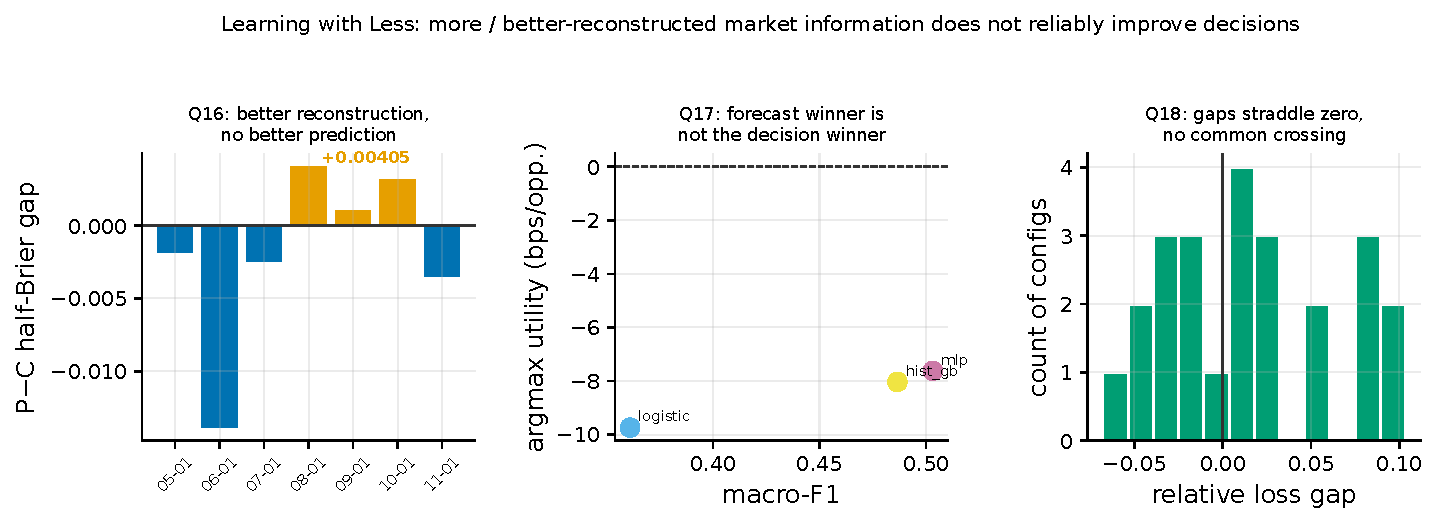
\includegraphics[width=\linewidth]{figures/fig_teaser.pdf}
\caption{\textbf{One instrument, three negative answers.}
We hold the model family, training budget, evaluation dates, and decision policy fixed
and vary only the information the learner sees, on real Hyperliquid data.
\textbf{Left (Q16):} augmenting a coarse predictor with \emph{more accurately
reconstructed} hidden book summaries does not lower prediction loss. On the August
breakout cohort it is $+0.00405$ half-Brier \emph{worse} than the coarse predictor.
\textbf{Center (Q17):} the model that wins on macro-F1 (\texttt{mlp}) is not the model
that wins on decisions. Every learned policy sits below the zero-utility line at
$5$ bps per side.
\textbf{Right (Q18):} the depth/history/delay effect straddles zero across $120$
model$\times$asset$\times$factor configurations, with no common crossing.}
\label{fig:teaser}
\end{figure}

We build that instrument and run it three ways on Hyperliquid perpetual-futures data
(Figure~\ref{fig:teaser}). Each study is a paired comparison in which only the observed
information changes. \textbf{Q16} asks whether reconstructing hidden order-book structure
improves the decision signal: we compare a coarse predictor, a predictor augmented with
reconstructed hidden summaries, and an observed-rich predictor, all trained and scored
identically. \textbf{Q17} asks whether forecast-quality rankings survive translation into
executable decisions: frozen forecasts from several model families pass through fixed
policies under explicit spread, latency, and cost assumptions. \textbf{Q18} asks whether
any fixed book depth, history length, or update delay is universally sufficient: a frozen
factorial varies each axis on matched dates. The headline is that all three answers are
negative, and they agree: better intermediate information does not reliably become better
decisions.

Our contributions are the following.
\begin{itemize}[leftmargin=1.4em]
\item \textbf{A matched information-intervention protocol} for real order-book data that
 fixes model, budget, dates, and policy and varies only the observed information, so the
 effect is read at the decision rather than at a forecasting score
 (Section~\ref{sec:setup}).
\item \textbf{A decision-grade negative for reconstruction (Q16):} across seven monthly
 breakout cohorts every hidden summary is reconstructed more accurately than a frozen
 baseline, yet the reconstruction-augmented predictor is $+0.00405$ half-Brier worse than
 the coarse predictor and $0.01762$ worse than a training-frequency baseline on the
 $691$-event August cohort. Controlled mechanism studies reproduce the same null
 (Section~\ref{sec:q16}).
\item \textbf{A forecast-then-decision reversal audit (Q17):} a multilayer perceptron
 beats logistic regression on macro-F1 by $0.142$ (BTC) and $0.097$ (ETH) while every
 learned policy loses money at $5$ bps per side. $0$ of $8$ protocol contrasts pass the
 joint gate (Section~\ref{sec:q17}).
\item \textbf{A sufficiency factorial (Q18):} no depth, history, or delay setting yields a
 common cross-asset benefit across $120$ fits, and the sign of the effect flips with
 model and asset, so no universal sufficiency threshold exists in this panel
 (Section~\ref{sec:q18}).
\item \textbf{A released, laptop-reproducible programme} of thirty curated experiment
 packages with source certification, provenance, and honest scientific status labels
 (Section~\ref{sec:synthesis}). An anonymized copy of the code, results, and this paper is
 available at \url{https://anonymous.4open.science/r/learning-with-less-C713}.
\end{itemize}

The result is not that information is worthless. It is that its value is conditional,
small, and easily destroyed by the policy and cost layer that any real decision must
cross. We argue this is the more useful thing to measure.

\section{Related work}
\label{sec:related_work}

\paragraph{Deep learning from the limit order book.} A large line predicts short-horizon
price moves directly from book states, from early convolutional and recurrent models
\citep{sirignano2016deep, zihao2018deeplob, zhang2018bdlob, nousi2018machine,
zheng2012price} through attention and information-persistence architectures
\citep{jung2024attention, briola2024hlob, lorenzo2022short} to generative and foundation
models of microstructure \citep{yanzhi2026m, xinpeng2026network, zihao2021deep} and to
representation-learning surveys and benchmarks of the book itself
\citep{zhong2025representation, ntakaris2017benchmark, briola2024deep}. This line asks how
well a model can predict. It holds the information fixed and varies the model. We invert
that: we hold the model fixed and vary the information, and we read the effect at a
decision rather than at a forecasting score.

\paragraph{Order-flow structure and queues.} A parallel line engineers ever finer views of
the book: multi-level and generalized order-flow imbalance
\citep{ke2019multi, rama2010price, su2021price, hu2025stochastic, bechler2014optimal}, the
dynamics of order positions and queues \citep{guo2015dynamics, cont2012order, toke2013order,
lipton2013trade}, and depth forecasting from the book \citep{libman2021forecasting}. These
works establish that finer structure carries statistical information. Our Q16 and Q18 ask
the next question, whether recovering that structure or paying for more of it changes a
decision, and find that on real data it usually does not.

\paragraph{Fill probability, queue position, and execution.} Whether an order fills, and at
what cost, has been modeled with survival analysis and state-dependent order flow
\citep{alvaro2023deep, lokin2024fill} and embedded in optimal-execution and market-impact
theory \citep{kato2014vwap, kato2009optimal, curato2014optimal, said2018market,
brokmann2014slow, lemhadri2018market, bechler2017order}. These give the mechanisms by which
book detail \emph{could} matter for a decision. Our finite-queue analysis (Section
\ref{sec:q16}) confirms the mechanism exists but is rare, and our reconstruction diagnostic
shows that recovering the hidden queue does not improve the fill/adverse/no-move decision.

\paragraph{Forecast quality versus decision value.} The gap between a good forecast and a
good decision is documented across domains: rank correlation between accuracy and decision
quality breaks down \citep{falezza2026when, raeth2025forecast}, statistical accuracy is a
weak proxy for economic value in electricity and energy markets
\citep{maciejowska2025statistical, kath2018value}, and decision-focused learning trains to
the decision precisely because training to the forecast is insufficient
\citep{wilder2018melding, zhou2024decision, silvestri2023score, tankov2021decision,
samuel2020information}. Proper-betting guarantees do exist under matched scoring rules and
liquidity conditions \citep{anri2026when}. Our Q17 supplies the matched market measurement
this line calls for: a frozen joint gate on real perpetual-futures data where the forecast
winner is not the decision winner.

\paragraph{Forecast evaluation and calibration.} Tools that evaluate forecasts across
decision thresholds, Murphy diagrams, the Triptych, consistent scoring functions, and
calibration diagnostics \citep{f2017murphy, timo2023evaluating, werner2015quantiles,
graziani2019probabilistic, loveday2023user, taggart2021point, allen2024tail,
bouallegue2015quantile}, already warn that one accuracy number hides decision-relevant
disagreement. We take the warning literally and measure the disagreement in basis points
under an explicit policy and cost model.

\paragraph{Benchmarks, leakage, and representation sufficiency.} Recent benchmarks probe
decision-time leakage and execution realism in learned trading
\citep{fan2026when, junyi2026beyond, nagy2025lob, cao2022dslob}, backtest correctness and
overfitting \citep{low2015correctness, koshiyama2019avoiding, pham2026algoxpert}, and
agent-based simulators for counterfactual evaluation \citep{dwarakanath2024abides,
backhouse2025painting}. On the theory side, decision-sufficient representations preserve the
optimal action rather than the input \citep{ye2026learning, walsh2026support}, and
information-theoretic limits bound what any predictor can extract
\citep{maurice2026forecastability}. Our released programme operationalizes this stance:
matched interventions, frozen gates, source certification, and honest status labels, so a
scoped negative is trustworthy rather than an artifact of leakage or a peeked date.

\section{The matched information-intervention instrument}
\label{sec:setup}

\paragraph{Principle.} Every study in this paper is one intervention: fix the model
family, the training budget, the train/validation/test date split, and the decision
policy, then change only the information the learner is allowed to observe. Anything that
would let a confound leak in, retuning per view, reusing a peeked date, or scoring a
view on its own clock, is held constant by construction. The comparison is paired at
the level of the event, so a difference is attributable to information, not to model
capacity or to luck on an easy day.

\paragraph{Data.} We use real Hyperliquid perpetual-futures observations. Q17 uses $30$
admitted native on-change best-bid/offer contracts across BTC and ETH over $15$ paired
calendar dates. Q18 uses $18$ admitted sampled-L2 receipt-clock contracts across BTC and
ETH over $9$ dates. The Q16 reconstruction diagnostic uses seven monthly BTC breakout and
rebound cohorts drawn from a certified development source. All feature construction,
normalization, and target definitions are training-only and frozen before any test date is
touched. A separate source-and-schema audit certifies event ordering and timing before an
experiment is allowed to run, so a comparison is admitted only when its inputs are valid. Raw market dumps are never redistributed, and each package ships checksums and acquisition
instructions instead.

\paragraph{Views and predictors (Q16).} We compare three predictors that differ only in
the information they encode. The \emph{coarse} predictor (C) sees an aggregate view. The
\emph{augmented} predictor (P) adds machine-reconstructed estimates of hidden book
summaries (queue sizes, depth imbalance, and near-touch depth in basis points). And the
\emph{observed-rich} predictor (R) sees the true rich summaries. All three share the model
family, the training budget, and the dates. We score a multiclass fill/adverse/no-move
target with a half-Brier loss (multiclass Brier divided by two), and we anchor every
learned arm against two reference baselines: a per-day \emph{uniform} prediction and a
\emph{training-frequency} prediction. If reconstruction has decision value, P must beat C
and clear the training-frequency reference.

\paragraph{Policies and costs (Q17).} Frozen forecasts from six model families (a prior,
logistic regression, gradient boosting, a multilayer perceptron, a random control, and an
oracle) pass through three fixed decision policies: an argmax direction policy, a
confidence-thresholded policy, and a scheduling policy over $12$-opportunity windows.
Utility is measured in basis points per opportunity under an explicit execution model
with a $100$ ms quote offset and a $5$ bps-per-side cost. The pre-registered joint gate
requires a model to show both a predictive advantage \emph{and} a utility reversal across
at least two policy families on six of eight paired dates before a forecast-to-decision
improvement is declared.

\paragraph{Factorial (Q18).} We cross book depth (one versus five levels), history
(instantaneous versus a longer window), and update delay (a current versus a delayed
view) and fit each cell with logistic regression, gradient boosting, and a multilayer
perceptron. The pre-declared reading is a common crossing: a universal sufficiency
threshold would make the same view win across both assets and all model families with
simultaneous day-clustered intervals. We report the relative-loss gap of the full
depth-plus-history view against the reduced view for every cell.

\paragraph{Soundness.} None of the three studies is allowed an outcome-driven tweak: the
plans are frozen before test dates are seen, warnings (for example neural fits that reach
their iteration cap) are preserved rather than suppressed, and a failure to certify
noninferiority is never reported as proof of insufficiency. The evidence we present is a
set of scoped negatives and controlled mechanisms, and we label each one by exactly what
it does and does not establish.

\section{Q16: reconstructing hidden structure does not improve the decision signal}
\label{sec:q16}

\textbf{Reconstructing the hidden book more accurately did not make the final prediction
better.} This is the paper's cleanest result and its most counterintuitive one. A coarse
limit-order-book view discards the individual resting orders behind an aggregate volume,
and a natural pipeline tries to recover them: estimate the hidden queue sizes and
near-touch depth, feed those estimates to the predictor, and expect a lift. We built that
pipeline on real BTC breakout and rebound cohorts and measured the lift directly.

\paragraph{Setup recap.} On seven monthly cohorts (May through November 2025) we compare
the coarse predictor C, the reconstruction-augmented predictor P, and the observed-rich
predictor R under the identical model, budget, and dates of Section~\ref{sec:setup},
scoring the multiclass target with half-Brier loss. Reconstruction quality is measured
separately: every hidden summary that P consumes is compared to a frozen target-mean
baseline, and on every cohort each summary is recovered \emph{more} accurately than that
baseline. The question is whether that recovered accuracy survives to the decision.

\paragraph{It does not.} Figure~\ref{fig:reconstruction} reads the August cohort, the
largest at $691$ events. The augmented predictor P scores a half-Brier loss of $0.35692$
against the coarse predictor's $0.35286$: augmenting with reconstructed structure made the
prediction \emph{worse} by $0.00405$. It is also $0.01762$ worse than the
training-frequency baseline, a predictor that ignores the current book entirely and
replays the training class mix. The observed-rich predictor R does not rescue the story:
it is $0.01793$ worse than C on the same cohort. Better recovered inputs, and even the
true rich inputs, bought a worse decision signal.

\begin{figure}[t]
\centering
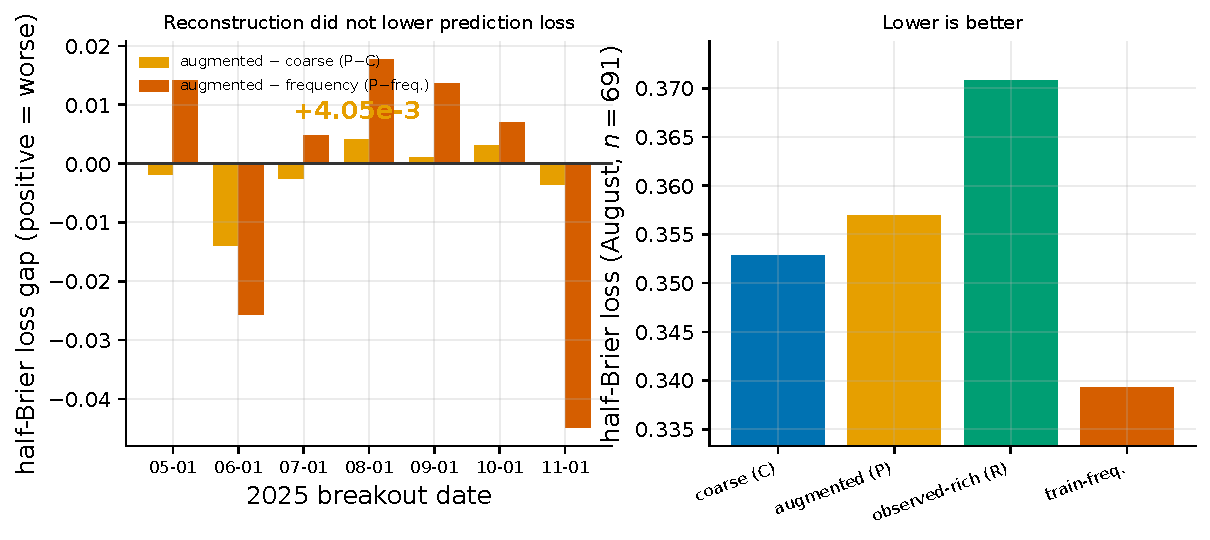
\includegraphics[width=\linewidth]{figures/fig_reconstruction.pdf}
\caption{\textbf{Q16: more accurate reconstruction, no better prediction.}
\textbf{Left:} per-date half-Brier loss gap of the augmented predictor P against the
coarse predictor C (positive means P is worse) and against the training-frequency
baseline. P is worse than the frequency baseline on the majority of dates. The August
cohort ($n=691$) is annotated at $+0.00405$.
\textbf{Right:} absolute August losses for coarse (C), augmented (P), observed-rich (R),
and training-frequency. Lower is better. Neither reconstruction nor the true rich view
beats coarse, and none beats the book-free frequency baseline.}
\label{fig:reconstruction}
\end{figure}

\paragraph{The pattern is not a single unlucky day.} Pooling the four August--November
breakout dates under equal-day weighting ($n=1749$), P remains above C ($+0.00118$
half-Brier) and R remains above C ($+0.00318$). No learned breakout arm beats the
training-frequency reference under event weighting, and on the earlier development dates
the learned arms lose to frequency as well. An earlier aggregate that had appeared to
favor rich depth disappeared once models were frozen and re-scored on held-out months:
the apparent gain was a class-mix and aggregation artifact, localized by a post-hoc
decomposition that separates the class-mixture term from the within-class term.

\paragraph{Controlled mechanism.} To check that this is not an estimation failure specific
to the market pipeline, we reproduce it in a controlled synthetic setting where the hidden
state and the optimal decision are known. There, restricted summaries incur $0.075$
decision regret, but a matched direct predictor and the posterior-restoration predictor
produce \emph{equal} decision coordinates: hidden-queue uncertainty matters, yet
reconstruction carries no isolated advantage over predicting the decision directly, and at
$512$ training draws the direct and distributional outputs coincide. A conditional shift
that is invisible in the observation marginal harms both approaches identically. The
mechanism is general: reconstruction spends capacity recovering structure that the
decision does not need.

\paragraph{The finite-queue special case.} The original Q16 question, can knowing the
\emph{count} and identity of individual orders narrow which fills are feasible?, has a
clean constructed answer that points the same way. In a finite FIFO model over $1000$
histories, aggregate volume alone leaves $59$ histories ambiguous, and adding displayed
order counts leaves $19$. Counts narrow the feasible outcome in $40$ of $1000$ histories.
The information is real but rare. On admitted native Hyperliquid observations the same
count-tightening was not established ($0$ of $961$ in the conditional cohort), and the
mandatory native-FIFO endpoint requires an order-lifecycle archive we located but have not
yet fully processed (Section~\ref{sec:synthesis}). The decision-relevance evidence for Q16
therefore rests on the reconstruction diagnostic above, where the answer is unambiguous:
recovering hidden structure did not help the decision.

\section{Q17: forecast-quality rankings do not survive the decision}
\label{sec:q17}

\textbf{The model that forecasts best is not the model that decides best.} A forecasting
score, macro-F1, log loss, direction accuracy, measures a statistical target, but a
trader acts through a policy under a spread, a latency, and a cost. Q17 asks whether the
ranking induced by the score survives translation into that action. We freeze forecasts
from six model families and push them through three fixed policies under an explicit
execution model (Section~\ref{sec:setup}), on $30$ native BBO contracts over $15$ paired
BTC/ETH dates, completing $22$ fits.

\paragraph{The forecast ranking is clear.} The multilayer perceptron is the best learned
forecaster on both assets: it improves macro-F1 over the logistic baseline by $0.142$ on
BTC and $0.097$ on ETH, with the BTC gain excluding zero on every one of the eight paired
dates. On the score alone, one would deploy the perceptron.

\paragraph{The decision ranking erases the win.} Figure~\ref{fig:q17} plots each model at
its forecast quality against its argmax utility at $5$ bps per side. Every learned policy
sits below the zero-utility line: on BTC the logistic policy returns $-9.74$ bps per
opportunity and the perceptron $-7.62$. On ETH the logistic policy returns $-9.96$ and the
perceptron $-8.15$. The perceptron loses \emph{less} than logistic regression, so the sign
of the forecast advantage is preserved in relative utility, but the absolute decision is
to trade at a loss, and the confidence policy's best move is to abstain to exactly zero.
The oracle itself, which knows the future label, still returns negative argmax utility
($-5.67$ BTC, $-5.46$ ETH) because the utility uses quote endpoints and assumed costs
rather than realized fills: even perfect foresight does not clear the cost layer under this
policy.

\begin{figure}[t]
\centering
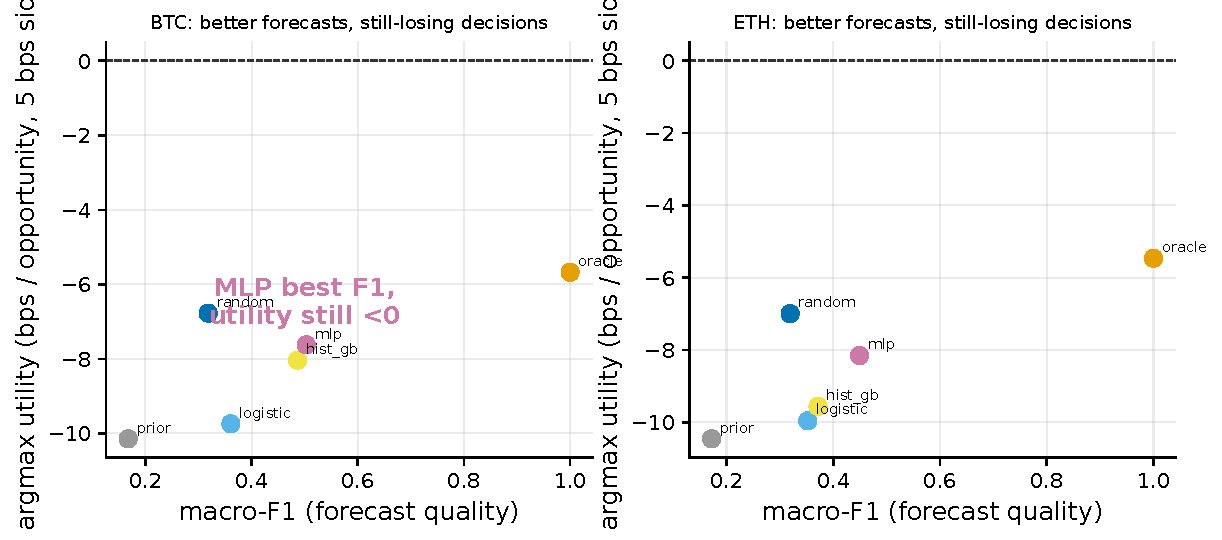
\includegraphics[width=\linewidth]{figures/fig_q17_forecast_decision.pdf}
\caption{\textbf{Q17: better forecasts, still-losing decisions.} Each point is a model
family placed at its macro-F1 (x) and its argmax utility in basis points per opportunity
at $5$ bps per side (y), for BTC (left) and ETH (right). Moving right (better forecasts)
does not move above the dashed zero-utility line: every learned policy trades at a loss,
and the forecast winner (\texttt{mlp}) is not a profitable decision.}
\label{fig:q17}
\end{figure}

\paragraph{The joint gate fails on every contrast.} The pre-registered criterion for
declaring a forecast-to-decision improvement requires both a predictive advantage and a
utility reversal across at least two policy families on six of eight dates. Of the eight
protocol contrasts (one macro-F1 and three utility contrasts per asset), $0$ pass. BTC
shows a significant macro-F1 gain but the confidence and scheduling contrasts fail their
thresholds, and all four ETH contrasts fail. The scheduling policy is negative on four of
eight dates for both assets. A forecast advantage that is real on the score is not a
decision advantage after the policy and cost layer intervene.

\paragraph{Why this is more than a restatement.} That scores and decisions can diverge is
known in principle \citep{falezza2026when, raeth2025forecast, f2017murphy,
timo2023evaluating}, and proper-betting guarantees exist under matched scoring rules and
liquidity conditions \citep{anri2026when}. Our contribution is the matched measurement on
real perpetual-futures data with a frozen joint gate: the divergence is not a corner case
produced by one arbitrary strategy, it is the outcome under the strongest learned
forecaster and three standard policies, and it holds on both assets. The forecasting
leaderboard and the trading leaderboard are different objects, and Q17 shows how far apart
they sit once real costs are paid.

\section{Q18: no fixed depth, history, or delay is universally sufficient}
\label{sec:q18}

\textbf{There is no single view that is enough for every decision.} Q18 tests the vendor's
implicit promise most directly: that a deeper, longer, fresher feed is uniformly better,
so a buyer can pick one sufficient configuration and stop paying for more. We cross book
depth (one versus five levels), history (instantaneous versus a longer window), and update
delay (current versus delayed) and fit every cell with three model families on $18$
sampled-L2 contracts over $9$ BTC/ETH dates, for $120$ fits.

\paragraph{The effect has no common sign.} Figure~\ref{fig:q18} shows the relative-loss
gap of the full depth-plus-history view against the reduced view for every
model$\times$asset$\times$factor cell on the transfer dates. A universal sufficiency
threshold would make these gaps line up on one side of zero. They do not. Adding depth
helps BTC logistic regression ($+0.077$ relative loss) but hurts the BTC perceptron with a
delayed view ($-0.049$). Adding depth helps ETH logistic regression ($+0.104$) while
removing history barely moves ETH gradient boosting. The signs flip with model and with
asset, and many simultaneous day-clustered intervals straddle zero, so the panel cannot
reject ``no effect'' for a fixed rule. A separate optimizer diagnostic sharpens the
disagreement: shallow inputs fit BTC better while deeper inputs fit ETH better, at both
$60$ and $600$ iterations, so the two assets ask for opposite feeds.

\begin{figure}[t]
\centering
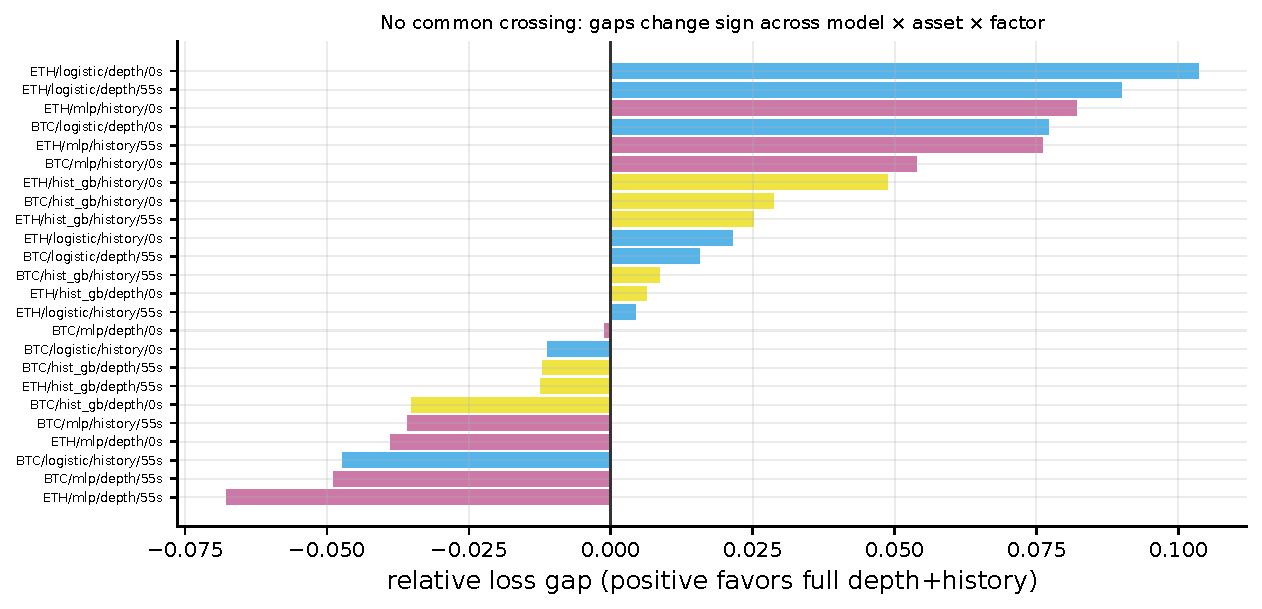
\includegraphics[width=\linewidth]{figures/fig_q18_no_crossing.pdf}
\caption{\textbf{Q18: no common crossing.} Relative-loss gap (full depth+history minus
reduced view. Positive favors the richer view) for every model$\times$asset$\times$factor
$\times$delay cell on the transfer dates, sorted. A universal sufficiency threshold would
put all bars on one side of zero. Instead the effect changes sign across configurations,
and its magnitude is small relative to the spread.}
\label{fig:q18}
\end{figure}

\paragraph{What the negative does and does not say.} It does not say depth is useless.
Some cells genuinely improve with more information, and the certified reading in a stricter
companion analysis (six asset--model combinations, both assets, at least two families
required) certifies a clock-induced change in $0$ of $6$ cases while explicitly refusing to
convert a failure-to-certify-noninferiority into a proof of insufficiency. What the panel
rejects is the \emph{simple} rule, ``five levels are always enough'' or ``freshness
always makes depth valuable'', that a one-size feed decision would need. Extra market
detail behaves like adding sensors to a control system: the sensors may carry information,
but a particular learner, sample, or timing alignment can fail to exploit it, and here the
exploitation fails inconsistently across exactly the axes a buyer would want to hold fixed.

\paragraph{Relation to representation-sufficiency theory.} Formal work defines
decision-sufficient representations as those that preserve the optimal action
\citep{ye2026learning, walsh2026support}, and depth-aware forecasting studies map
predictive value to book levels \citep{briola2024hlob, briola2024deep}. Our panel is the
empirical complement: a classifier plateau cannot estimate a theoretical sufficient
dimension, but it can show that no fixed observable configuration is sufficient across
assets and models on real data. The sufficiency question is therefore conditional by
nature, and a leaderboard that reports one average curve hides the sign changes that
decide whether a feed is worth buying.

\section{Synthesis: information value is conditional, small, and policy-fragile}
\label{sec:synthesis}

\textbf{Three questions, asked with one instrument, returned the same answer.} Read
together, Q16, Q17, and Q18 rule out the monotone premise that organizes much of applied
market-microstructure learning. Reconstructing hidden structure did not improve the
decision signal (Q16). The best forecaster was not the best decider (Q17). And no fixed
observable configuration was universally sufficient (Q18). The common cause is visible
once the studies are aligned: value that is real at the level of a statistical target, a recovered queue size, a higher macro-F1, a deeper book, is small in magnitude and is
absorbed or reversed by the policy and cost layer that separates a prediction from a
decision. This is why we measure at the decision. A programme that had stopped at
reconstruction RMSE, at macro-F1, or at an averaged depth curve would have reported three
positive results. Measured at the decision, all three are negative.

\paragraph{The reusable object.} The contribution readers can depend on is the
\emph{matched information-intervention protocol}: freeze model, budget, dates, and policy. Vary only the observed information. Read the effect at the decision under an explicit cost
model. And refuse outcome-driven tweaks. The protocol is what turns ``does richer data
help?'' into a falsifiable measurement, and it transfers beyond these three questions to
any setting where a feed is bought on the promise of downstream value.

\paragraph{The released programme.} We release thirty curated experiment packages spanning
the three real-data studies, controlled simulator mechanisms, breakout/rebound cohorts,
temporal-persistence checks, and source-and-schema certification. Each package carries its
question, method, compact results, figures, provenance, and an explicit scientific-status
label, and each is laptop-reproducible from a license-clean smoke fixture. Raw market
dumps are never redistributed. The labels are load-bearing: a completed software check, a
valid scientific negative, an inconclusive run, and a blocked empirical objective are kept
distinct rather than rounded up to ``done.''

\paragraph{One honest open endpoint.} The strictest form of Q16, native-FIFO count
tightening on a fully admitted order-lifecycle cohort, is not yet computed. We located
the exact source (an open December 2025 Level-4 Hyperliquid archive of $195.3$ GB with
$744$ hourly files per order archive) and a bounded washout audit over $11$ complete hours
covered $32{,}633{,}820$ events, observing $11{,}328$ legacy order identifiers of which
$148$ were still first seen in hour $10$. Observed-lifecycle coverage reached
$99.92985\%$, but true live-book completeness remains unidentified, so we do not claim the
native-FIFO endpoint. We flag this rather than paper over it, and the decision-relevance
conclusion for Q16 stands on the reconstruction diagnostic, which needs no such admission.

\section{Limitations}
\label{sec:limitations}

We state the boundaries of the evidence plainly, because a negative result is only as
useful as its scope is honest.

\textbf{Scope of the negatives.} The three studies are scoped, not universal. Q17 covers
two assets and eight paired dates under a quote-based utility that uses quote endpoints and
assumed costs. It does not observe realized fills, endogenous market impact, funding, or
queue priority, so it is a decision-utility statement, not a live-trading profitability
statement. Q18 uses sampled-L2 receipt-clock data over nine dates. Its date panel is small
and its intervals are wide, so it rejects a simple sufficiency rule rather than proving
that depth never helps. Q16's reconstruction diagnostic uses development-exposed dates and
is descriptive rather than a pristine prospective holdout.

\textbf{Data realism.} Provider receipt time is uncalibrated against exchange time, and the
sampled-L2 feed does not establish native queue priority or calibrated latency. Where an
entity or feed could not be certified, the corresponding claim is withheld. The
native-FIFO Q16 endpoint (Section~\ref{sec:synthesis}) is the clearest such withholding.

\textbf{Estimation confounds.} Several neural fits reached their fixed iteration budget,
and their warnings are preserved rather than suppressed. Full-depth neural underperformance
can therefore reflect an optimization limit rather than an information limit. Because
changing only that family cannot rescue a result that requires agreement across families,
we do not lean on any single neural cell.

\textbf{What we do not claim.} We do not claim that information is worthless, that richer
feeds should never be purchased, or that these negatives generalize to other venues,
horizons, or asset classes. We claim that, measured at the decision with everything else
held fixed, the value of more and better-reconstructed market information was small,
conditional, and fragile to the policy and cost layer, across three questions on real
data.

\section{Conclusion}
\label{sec:conclusion}

We asked whether more granular and more accurately reconstructed market information buys
better decisions, and across three matched studies on real Hyperliquid data the answer was
no. Reconstructing hidden book structure left the decision signal no better and often worse, on $691$ August breakout events the reconstruction-augmented predictor was $0.00405$
half-Brier worse than the coarse predictor and $0.01762$ worse than a book-free frequency
baseline. The best forecaster was not the best decider: a perceptron won macro-F1 by
$0.142$ (BTC) and $0.097$ (ETH) yet every learned policy lost money at $5$ bps per side,
and $0$ of $8$ protocol contrasts passed the joint gate. And no fixed depth, history, or
delay was universally sufficient: the effect changed sign across $120$ fits.

The through line is that information value lives at the decision, is small there, and is
easily undone by the policy and cost layer, so that is where it should be measured. The
reusable contribution is the matched information-intervention protocol and a released,
laptop-reproducible programme of thirty honestly labeled experiment packages. Learning with less
is often not a compromise. On these questions it was indistinguishable from, or better
than, learning with more \citep{ye2026learning, falezza2026when}.


\clearpage
\typeout{MAIN-TEXT-ENDS-ON-\the\numexpr\value{page}-1\relax}

\bibliographystyle{iclr2027_conference}
\bibliography{references}

\clearpage
\appendix
\typeout{APPENDIX-BEGINS-ON-\thepage}
\section{Notation, metrics, and definitions}
\label{app:notation}

\paragraph{Predictors.} \emph{Coarse (C)} sees an aggregate order-book view. \emph{Augmented
(P)} adds machine-reconstructed estimates of hidden book summaries (queue sizes, depth
imbalance, near-touch depth in basis points) to the coarse view. \emph{Observed-rich (R)} sees
the true rich summaries. All three share the model family, training budget, and dates. Only the
observed information differs.

\paragraph{Targets.} The reconstruction study scores a three-class target, fill (F), adverse
(A), no-move (N), with a half-Brier loss, defined as the multiclass Brier score divided by
two so that a uniform three-class prediction has a fixed reference value. Q17 discretizes a
short-horizon mid-quote move into up/down/flat and reports macro-F1. Q18 reports a relative-loss
gap, the fractional change in loss of the full depth-plus-history view against a reduced view.

\paragraph{Baselines.} The \emph{uniform} baseline predicts each class with equal probability
per day. The \emph{training-frequency} baseline predicts the training class mix and ignores the
current book. It is the key reference, because a predictor that cannot beat it has extracted no
usable book information. The \emph{oracle} in Q17 has access to the realized label and bounds
the best achievable decision utility under the policy and cost model.

\paragraph{Policies (Q17).} The \emph{argmax} policy acts on the highest-probability direction. The \emph{confidence} policy acts only above a fixed probability threshold and otherwise
abstains. The \emph{scheduling} policy allocates activity across a $12$-opportunity window.
Utility is in basis points per opportunity (argmax, confidence) or per window (scheduling), at
a $5$ bps-per-side cost and a $100$ ms quote-offset latency.

\paragraph{Gates.} Q17's joint gate requires a predictive advantage and a utility reversal
across at least two policy families on six of eight paired dates. Q18's certified companion
requires own-clock inferiority and inherited-clock noninferiority on both assets and at least
two model families. Both gates are frozen before test dates are read.

\paragraph{Per-class detail.} Table~\ref{tab:augclassreb} gives the August rebound cohort's
per-class breakdown, the companion to Table~\ref{tab:augclass}. The same pattern holds, the
augmented and rich predictors move the predicted probabilities but not the decision-relevant
losses.

\begin{table}[h]\centering
\caption{August rebound cohort ($n=668$): per-class predicted probability and per-class
half-Brier loss by method. Source: \texttt{experiments/results/e264\_figure\_source.json}.}
\label{tab:augclassreb}
\begin{tabular}{lrrrrrrr}
\toprule
method & $q_F$ & $q_A$ & $q_N$ & $\ell_F$ & $\ell_A$ & $\ell_N$ & total \\
\midrule
C & 0.089820 & 0.534431 & 0.375749 & 0.727097 & 0.282014 & 0.251431 & 0.310500 \\
P & 0.089820 & 0.534431 & 0.375749 & 0.727468 & 0.289412 & 0.239786 & 0.310111 \\
R & 0.089820 & 0.534431 & 0.375749 & 0.759518 & 0.331935 & 0.234081 & 0.333572 \\
onehot-F & 0.089820 & 0.534431 & 0.375749 & 0.000000 & 1.000000 & 1.000000 & 0.910180 \\
onehot-A & 0.089820 & 0.534431 & 0.375749 & 1.000000 & 0.000000 & 1.000000 & 0.465569 \\
onehot-N & 0.089820 & 0.534431 & 0.375749 & 1.000000 & 1.000000 & 0.000000 & 0.624251 \\
uniform & 0.089820 & 0.534431 & 0.375749 & 0.333333 & 0.333333 & 0.333333 & 0.333333 \\
train-frequency & 0.089820 & 0.534431 & 0.375749 & 0.643522 & 0.254912 & 0.253237 & 0.289188 \\
\bottomrule
\end{tabular}\end{table}


\section{Q16 reconstruction study: full results}
\label{app:recon}

This appendix expands Section~\ref{sec:q16}. The reconstruction study compares three
predictors that differ only in the information they encode, coarse (C), reconstruction
augmented (P), and observed rich (R), against two reference baselines (a per-day uniform
prediction and a training-frequency prediction), scoring a three-class fill/adverse/no-move
target with half-Brier loss (multiclass Brier divided by two). All arms share the model
family, the training budget, and the calendar dates. Only the observed information differs.

\paragraph{Per-date losses.} Table~\ref{tab:recon} lists every predictor's half-Brier loss
for each monthly cohort, together with the two decision-relevant gaps: P$-$C (does
augmenting with reconstructed structure beat the coarse view?) and P$-$frequency (does it
beat a book-free baseline?). On the August breakout cohort ($n=691$) the augmented predictor P
scores a half-Brier loss of $0.35692$, against the coarse predictor's $0.35286$ and the
training-frequency baseline's $0.33930$. The gap to coarse is $+0.00405$ and the gap to
frequency is $+0.01762$: the augmented predictor is worse on both comparisons. The pattern is not confined to August. Across the
breakout cohorts the augmented predictor fails to beat the training-frequency baseline on
the majority of dates, and the observed-rich predictor R does no better, confirming that
the failure is about the decision target rather than about reconstruction error.

\begin{longtable}{llrrrrrrrr}
\caption{Q16 reconstruction study: per-date half-Brier loss by predictor, with the two
decision-relevant gaps. C = coarse, P = reconstruction-augmented, R = observed-rich.
Positive gaps mean the augmented predictor is worse. All values from
\texttt{experiments/results/e264\_figure\_source.json}.}
\label{tab:recon}\\
\toprule
family & date & $n$ & C & P & R & uniform & train-freq. & P$-$C & P$-$freq. \\
\midrule
\endfirsthead
\toprule
family & date & $n$ & C & P & R & uniform & train-freq. & P$-$C & P$-$freq. \\
\midrule
\endhead
\bottomrule
\endfoot
breakout & 2025-05-01 & 372 & 0.310878 & 0.309019 & 0.302571 & 0.333333 & 0.294974 & -0.001858 & 0.014046 \\
breakout & 2025-06-01 & 155 & 0.235191 & 0.221313 & 0.211069 & 0.333333 & 0.247009 & -0.013879 & -0.025697 \\
breakout & 2025-07-01 & 247 & 0.288472 & 0.286019 & 0.276986 & 0.333333 & 0.281304 & -0.002453 & 0.004715 \\
breakout & 2025-08-01 & 691 & 0.352863 & 0.356918 & 0.370796 & 0.333333 & 0.339301 & 0.004054 & 0.017616 \\
breakout & 2025-09-01 & 594 & 0.299716 & 0.300729 & 0.302344 & 0.333333 & 0.287154 & 0.001013 & 0.013575 \\
breakout & 2025-10-01 & 360 & 0.283368 & 0.286514 & 0.279983 & 0.333333 & 0.279556 & 0.003145 & 0.006958 \\
breakout & 2025-11-01 & 104 & 0.203500 & 0.199986 & 0.199041 & 0.333333 & 0.244839 & -0.003514 & -0.044853 \\
rebound & 2025-05-01 & 317 & 0.300703 & 0.293038 & 0.303007 & 0.333333 & 0.283472 & -0.007665 & 0.009566 \\
rebound & 2025-06-01 & 122 & 0.273435 & 0.272781 & 0.273255 & 0.333333 & 0.260157 & -0.000654 & 0.012624 \\
rebound & 2025-07-01 & 195 & 0.281781 & 0.285348 & 0.290173 & 0.333333 & 0.267969 & 0.003567 & 0.017379 \\
rebound & 2025-08-01 & 668 & 0.310500 & 0.310111 & 0.333572 & 0.333333 & 0.289188 & -0.000389 & 0.020923 \\
rebound & 2025-09-01 & 574 & 0.304925 & 0.304402 & 0.298784 & 0.333333 & 0.279154 & -0.000523 & 0.025248 \\
rebound & 2025-10-01 & 311 & 0.301289 & 0.300011 & 0.314831 & 0.333333 & 0.276532 & -0.001277 & 0.023480 \\
rebound & 2025-11-01 & 80 & 0.259826 & 0.252390 & 0.280369 & 0.333333 & 0.263518 & -0.007436 & -0.011127 \\
\end{longtable}


\paragraph{Decomposition.} A post-hoc decomposition separates each loss gap into a
class-mixture term (differences in the realized class frequencies across cohorts) and a
within-class term (differences in per-class loss). The earlier aggregate that had appeared
to favor rich depth is localized to the class-mixture term and to equal-versus-pooled
day weighting. Under event weighting, no learned breakout arm beats the training-frequency
reference. This is why we report the gap under a fixed weighting and against an explicit
baseline rather than as a single aggregate number: the aggregate is exactly where the
artifact hid.

\paragraph{Per-class breakdown of the headline cohort.} Table~\ref{tab:augclass} opens the
August cohort by class. The augmented predictor P and the observed-rich predictor R shift the
predicted class probabilities toward the recovered structure, but the per-class losses do not
improve over the coarse predictor C on the classes that matter for the decision. The total loss
rises accordingly. The one-hot rows confirm that the target is genuinely three-way and that no
single class dominates the loss, so the null is not an artifact of a degenerate label.

\begin{table}[h]\centering
\caption{August breakout cohort ($n=691$): per-class predicted probability ($q$) and per-class
half-Brier loss ($\ell$) for each method, with total loss. Classes are fill (F), adverse (A),
and no-move (N). Source: \texttt{experiments/results/e264\_figure\_source.json}.}
\label{tab:augclass}
\begin{tabular}{lrrrrrrr}
\toprule
method & $q_F$ & $q_A$ & $q_N$ & $\ell_F$ & $\ell_A$ & $\ell_N$ & total \\
\midrule
C & 0.367583 & 0.231548 & 0.400868 & 0.375428 & 0.680592 & 0.142871 & 0.352863 \\
P & 0.367583 & 0.231548 & 0.400868 & 0.400633 & 0.688576 & 0.125261 & 0.356918 \\
R & 0.367583 & 0.231548 & 0.400868 & 0.440539 & 0.708046 & 0.112043 & 0.370796 \\
onehot-F & 0.367583 & 0.231548 & 0.400868 & 0.000000 & 1.000000 & 1.000000 & 0.632417 \\
onehot-A & 0.367583 & 0.231548 & 0.400868 & 1.000000 & 0.000000 & 1.000000 & 0.768452 \\
onehot-N & 0.367583 & 0.231548 & 0.400868 & 1.000000 & 1.000000 & 0.000000 & 0.599132 \\
uniform & 0.367583 & 0.231548 & 0.400868 & 0.333333 & 0.333333 & 0.333333 & 0.333333 \\
train-frequency & 0.367583 & 0.231548 & 0.400868 & 0.366264 & 0.578116 & 0.176634 & 0.339301 \\
\bottomrule
\end{tabular}\end{table}


\paragraph{Controlled mechanism.} The synthetic control of Section~\ref{sec:q16} places the
same question in a setting with a known hidden state and a known optimal action. Restricted
summaries incur $0.075$ decision regret relative to the full-information optimum, but a
matched direct predictor and a posterior-restoration predictor produce equal decision
coordinates, and at $512$ training draws their outputs coincide. The lesson transfers: when
the decision does not require the hidden structure, reconstructing it spends capacity
without changing the action, and when a conditional shift is invisible in the observation
marginal it harms both approaches equally. Reconstruction is therefore neither a free lunch
nor a targeted fix. It is orthogonal to the decision unless the decision needs precisely the
recovered coordinate.

\paragraph{Finite-queue special case.} The constructed finite FIFO analysis isolates the
narrowest version of the original Q16 question: can the displayed \emph{count} of resting
orders narrow which fills are feasible beyond what aggregate volume already implies? Over
$1000$ enumerated histories, aggregate volume leaves $59$ ambiguous and adding counts leaves
$19$. Counts strictly narrow the feasible outcome in $40$ histories. The tightening is real
but rare, and on the admitted native Hyperliquid cohort the same tightening was not observed
($0$ of $961$ primary. $0$ of $962$ in a postrun completion check), consistent with the
reconstruction diagnostic: the extra information exists but seldom changes the decision.

\section{Q17 forecast-to-decision study: protocol and full results}
\label{app:q17}

\paragraph{Data and features.} Q17 uses $30$ admitted native on-change best-bid/offer
contracts across BTC and ETH over $15$ paired calendar dates. Features are past-only quote
statistics computed on the receipt clock. The target is the sign of a short-horizon
mid-quote move discretized into up/down/flat. Feature construction and normalization are
fit on the training portion only and frozen before any test date is scored. Six model
families produce frozen forecasts: a class-prior baseline, logistic regression, gradient
boosting, a multilayer perceptron, a random control, and an oracle with access to the
realized label.

\paragraph{Policies and utility.} Each frozen forecast passes through three fixed policies.
The \emph{argmax} policy takes the highest-probability direction. The \emph{confidence}
policy acts only above a fixed probability threshold and otherwise abstains. The
\emph{scheduling} policy allocates activity across a $12$-opportunity window. Utility is
computed with inverse-contract price arithmetic and scenario fees at a $5$ bps-per-side
cost and a $100$ ms quote-offset latency. Utility uses quote endpoints and assumed costs. It does not observe realized fills, funding, or endogenous impact, so it is a decision
utility, not a realized profit.

\paragraph{Joint gate.} A forecast-to-decision improvement is declared only when a model
shows both a predictive advantage and a utility reversal across at least two policy families
on six of eight paired dates. Table~\ref{tab:q17primary} reports the four primary contrasts
per asset (one macro-F1 and three utility contrasts). No contrast passes: the BTC macro-F1
gain is significant, but the confidence and scheduling contrasts fail, and all four ETH
contrasts fail. The confidence policy collapses to zero utility (abstain) for every learned
model, and the scheduling contrast is negative on four of eight dates for both assets.

\begin{table}[h]\centering
\caption{Q17 primary contrasts (MLP minus logistic) with bootstrap intervals over eight
paired dates. Source: \texttt{experiments/results/q17\_primary\_contrasts.csv}. No
contrast passes the joint gate.}
\label{tab:q17primary}
\begin{tabular}{llrrrr}
\toprule
asset & metric & mean & 95\% interval & neg. dates & passed \\
\midrule
BTC & macro\_f1 & 0.142103 & [0.039529, 0.244677] & 0 & \checkmark \\
BTC & argmax & 2.122375 & [0.292744, 3.952005] & 0 & $\times$ \\
BTC & confidence & 0.000000 & [0.000000, 0.000000] & 0 & $\times$ \\
BTC & scheduling & 0.025961 & [-0.102278, 0.154200] & 4 & $\times$ \\
ETH & macro\_f1 & 0.097081 & [0.006888, 0.187274] & 1 & $\times$ \\
ETH & argmax & 1.801718 & [0.096671, 3.506765] & 1 & $\times$ \\
ETH & confidence & 0.000000 & [0.000000, 0.000000] & 0 & $\times$ \\
ETH & scheduling & -0.070943 & [-0.524662, 0.382776] & 4 & $\times$ \\
\bottomrule
\end{tabular}
\end{table}


\begin{table}[h]\centering
\caption{Q17 absolute performance by model family. Utility in basis points per
opportunity (argmax, confidence) or per 12-opportunity window (scheduling) at 5 bps per
side. Source: \texttt{experiments/results/q17\_figure\_data.json}.}
\label{tab:q17abs}
\begin{tabular}{llrrrr}
\toprule
asset & model & macro-F1 & argmax & confidence & scheduling \\
\midrule
BTC & prior & 0.167633 & -10.143430 & 0.000000 & -0.087832 \\
BTC & logistic & 0.361085 & -9.741636 & 0.000000 & 0.680911 \\
BTC & hist\_gb & 0.486577 & -8.034500 & 0.000000 & 0.531820 \\
BTC & mlp & 0.503188 & -7.619262 & 0.000000 & 0.706872 \\
BTC & random & 0.318313 & -6.772006 & 0.000000 & -0.080510 \\
BTC & oracle & 1.000000 & -5.673321 & 0.000000 & 1.997775 \\
ETH & prior & 0.171960 & -10.455921 & 0.000000 & -0.108507 \\
ETH & logistic & 0.352168 & -9.956131 & 0.000000 & 0.903621 \\
ETH & hist\_gb & 0.371520 & -9.559819 & 0.000000 & 0.797432 \\
ETH & mlp & 0.449249 & -8.154412 & 0.000000 & 0.832678 \\
ETH & random & 0.319194 & -6.992946 & 0.000000 & -0.080479 \\
ETH & oracle & 1.000000 & -5.461902 & 0.000000 & 2.752498 \\
\bottomrule
\end{tabular}
\end{table}


\begin{table}[h]\centering
\caption{Q17 per-date macro-F1 advantage of the MLP over logistic regression, by paired date,
with the mean. Source: \texttt{experiments/results/q17\_figure\_data.json}.}
\label{tab:q17days}
\begin{tabular}{lrrrrrrrrr}
\toprule
asset & d1 & d2 & d3 & d4 & d5 & d6 & d7 & d8 & mean \\
\midrule
BTC & 0.223477 & 0.072209 & 0.265424 & 0.076891 & 0.089394 & 0.088852 & 0.194926 & 0.125649 & \textbf{0.142103} \\
ETH & -0.001203 & 0.073973 & 0.190915 & 0.060807 & 0.086582 & 0.080443 & 0.196469 & 0.088661 & \textbf{0.097081} \\
\bottomrule
\end{tabular}\end{table}


Table~\ref{tab:q17days} gives the per-date macro-F1 advantage: the BTC gain is positive on all
eight dates (hence the significant contrast), while the ETH gain is negative on one date, which
is why the ETH predictive contrast is weaker even though its mean is positive.

\paragraph{Absolute performance.} Table~\ref{tab:q17abs} gives the absolute macro-F1 and
per-policy utility for every model family. The ordering by macro-F1 (oracle $>$ mlp $>$
hist\_gb $>$ logistic $>$ random $>$ prior) does not match the ordering by argmax utility,
and every learned argmax utility is negative. The oracle's own argmax utility is negative
($-5.67$ BTC, $-5.46$ ETH), which bounds how much the cost layer alone removes: even a
perfect direction forecast trades at a loss under this policy and cost model. This is the
quantitative core of the section: the forecasting leaderboard and the decision leaderboard
are different orderings, and the gap is large enough to invert the deployment choice.

\paragraph{Sensitivity across later dates.} A frozen follow-up sweeps fixed cost and latency
scenarios on additional dates without changing the gate. The per-policy utility ranges
remain policy-dependent and continue to straddle zero for the confidence and scheduling
families, so the negative is not an artifact of one cost assumption. We report ranges rather
than a single tuned scenario precisely to avoid selecting the cost point that would flip the
conclusion.

\section{Q18 sufficiency factorial: protocol and full results}
\label{app:q18}

\paragraph{Design.} Q18 crosses three information axes, book depth (one versus five
levels), history (instantaneous versus a longer window), and update delay (a current view
versus a view delayed by $55$ seconds), and fits each cell with logistic regression,
gradient boosting, and a multilayer perceptron on $18$ admitted sampled-L2 receipt-clock
contracts across BTC and ETH over $9$ dates, for $120$ fits. The response is the
relative-loss gap of the full depth-plus-history view against the reduced view. A positive
gap favors the richer view. Normalization and feature transforms are training-only.

\paragraph{No common crossing.} Table~\ref{tab:q18} lists every cell for both the pilot and
transfer stages. A universal sufficiency threshold would place all transfer gaps on one side
of zero with simultaneous intervals excluding it. Instead the gaps change sign across model,
asset, and factor: on transfer dates BTC logistic regression gains $+0.077$ from depth while
the BTC perceptron with a delayed view loses $-0.049$. ETH logistic regression gains $+0.104$
from depth while ETH gradient boosting with a delayed view is slightly negative. Many
simultaneous upper bounds sit on the opposite side of the point estimate, so the panel cannot
reject ``no effect'' for a fixed rule.

\begin{longtable}{lllllrr}
\caption{Q18 depth/history/delay factorial: relative-loss gap of the full depth+history
view against the reduced view (positive favors the richer view), with simultaneous upper
bounds on transfer dates. Source: \texttt{experiments/results/q18\_contrasts.csv}.}
\label{tab:q18}\\
\toprule
stage & asset & model & delay & factor & rel.\ loss & sim.\ upper \\
\midrule
\endfirsthead
\toprule
stage & asset & model & delay & factor & rel.\ loss & sim.\ upper \\
\midrule
\endhead
\bottomrule
\endfoot
pilot & BTC & logistic & 0 & depth & 0.009179 & -- \\
pilot & BTC & logistic & 0 & history & 0.020433 & -- \\
pilot & BTC & logistic & 55 & depth & -0.006219 & -- \\
pilot & BTC & logistic & 55 & history & 0.012249 & -- \\
pilot & BTC & hist\_gb & 0 & depth & 0.015945 & -- \\
pilot & BTC & hist\_gb & 0 & history & 0.022297 & -- \\
pilot & BTC & hist\_gb & 55 & depth & 0.020958 & -- \\
pilot & BTC & hist\_gb & 55 & history & 0.019063 & -- \\
pilot & ETH & logistic & 0 & depth & -0.003899 & -- \\
pilot & ETH & logistic & 0 & history & -0.011585 & -- \\
pilot & ETH & logistic & 55 & depth & -0.056422 & -- \\
pilot & ETH & logistic & 55 & history & -0.016132 & -- \\
pilot & ETH & hist\_gb & 0 & depth & 0.078818 & -- \\
pilot & ETH & hist\_gb & 0 & history & 0.021399 & -- \\
pilot & ETH & hist\_gb & 55 & depth & 0.008940 & -- \\
pilot & ETH & hist\_gb & 55 & history & 0.019923 & -- \\
transfer & BTC & logistic & 0 & depth & 0.077166 & 0.239233 \\
transfer & BTC & logistic & 0 & history & -0.011160 & 0.043219 \\
transfer & BTC & logistic & 55 & depth & 0.015667 & 0.070315 \\
transfer & BTC & logistic & 55 & history & -0.047349 & 0.013859 \\
transfer & BTC & hist\_gb & 0 & depth & -0.035137 & 0.014592 \\
transfer & BTC & hist\_gb & 0 & history & 0.028600 & 0.035509 \\
transfer & BTC & hist\_gb & 55 & depth & -0.011948 & 0.016189 \\
transfer & BTC & hist\_gb & 55 & history & 0.008541 & 0.011751 \\
transfer & BTC & mlp & 0 & depth & -0.001089 & 0.083898 \\
transfer & BTC & mlp & 0 & history & 0.053874 & 0.140525 \\
transfer & BTC & mlp & 55 & depth & -0.048831 & -0.026603 \\
transfer & BTC & mlp & 55 & history & -0.035745 & 0.071483 \\
transfer & ETH & logistic & 0 & depth & 0.103533 & 0.303054 \\
transfer & ETH & logistic & 0 & history & 0.021481 & 0.080885 \\
transfer & ETH & logistic & 55 & depth & 0.089966 & 0.218659 \\
transfer & ETH & logistic & 55 & history & 0.004337 & 0.084905 \\
transfer & ETH & hist\_gb & 0 & depth & 0.006368 & 0.112091 \\
transfer & ETH & hist\_gb & 0 & history & 0.048809 & 0.068430 \\
transfer & ETH & hist\_gb & 55 & depth & -0.012304 & -0.008693 \\
transfer & ETH & hist\_gb & 55 & history & 0.025069 & 0.048440 \\
transfer & ETH & mlp & 0 & depth & -0.038786 & 0.203815 \\
transfer & ETH & mlp & 0 & history & 0.082120 & 0.134936 \\
transfer & ETH & mlp & 55 & depth & -0.067779 & 0.148440 \\
transfer & ETH & mlp & 55 & history & 0.075997 & 0.140244 \\
\end{longtable}


\paragraph{Optimizer diagnostic.} A separate check varies the neural optimizer budget to
rule out a pure underfitting explanation. Shallow inputs fit BTC better while deeper inputs
fit ETH better, at both $60$ and $600$ iterations. The asset-dependent direction survives the
budget change, so it is not merely an artifact of an unconverged fit. Several neural cells
did reach their iteration cap, and their warnings are preserved. Because a universal rule
would require agreement across model families, no single neural cell can establish or rescue
the result.

\begin{table}[h]\centering
\caption{Q18 optimizer diagnostic: own-clock loss at depth 1 and depth 5 by asset and neural
budget. A positive shallow-minus-deep value means shallow inputs fit better. Source:
\texttt{experiments/results/q18\_figure\_data.json}.}
\label{tab:q18opt}
\begin{tabular}{lrrrr}
\toprule
asset & budget & depth-1 loss & depth-5 loss & shallow $-$ deep \\
\midrule
BTC & 60 & 0.307662 & 0.314045 & -0.006383 \\
BTC & 600 & 0.307170 & 0.316755 & -0.009585 \\
ETH & 60 & 0.291022 & 0.277982 & 0.013041 \\
ETH & 600 & 0.289594 & 0.281961 & 0.007633 \\
\bottomrule
\end{tabular}\end{table}


Table~\ref{tab:q18opt} gives the optimizer diagnostic in full: shallow inputs fit BTC better
(negative shallow-minus-deep) while deeper inputs fit ETH better (positive), at both budgets.
Table~\ref{tab:q18daily} shows the per-date components of the transfer-stage gaps, and makes
the instability concrete: within a single cell the daily gap changes sign across dates, so the
cell-level average is an average over disagreement rather than a stable effect.

\begin{longtable}{llllrrr}
\caption{Q18 per-date relative-loss gaps (transfer stage): the first three daily components of
each cell, showing how the sign varies day to day. Source:
\texttt{experiments/results/q18\_figure\_data.json}.}
\label{tab:q18daily}\\
\toprule
asset & model & delay & factor & day 1 & day 2 & day 3 \\
\midrule
\endfirsthead
\toprule
asset & model & delay & factor & day 1 & day 2 & day 3 \\
\midrule
\endhead
\bottomrule
\endfoot
BTC & logistic & 0 & depth & -0.029221 & 0.021485 & 0.239233 \\
BTC & logistic & 0 & history & 0.043219 & 0.006853 & -0.083553 \\
BTC & logistic & 55 & depth & -0.012472 & -0.010842 & 0.070315 \\
BTC & logistic & 55 & history & 0.013859 & -0.031358 & -0.124548 \\
BTC & hist\_gb & 0 & depth & -0.064672 & -0.055331 & 0.014592 \\
BTC & hist\_gb & 0 & history & 0.029717 & 0.035509 & 0.020573 \\
BTC & hist\_gb & 55 & depth & -0.031816 & -0.020217 & 0.016189 \\
BTC & hist\_gb & 55 & history & 0.008076 & 0.005796 & 0.011751 \\
BTC & mlp & 0 & depth & -0.060982 & -0.026183 & 0.083898 \\
BTC & mlp & 0 & history & 0.140525 & 0.124402 & -0.103304 \\
BTC & mlp & 55 & depth & -0.060315 & -0.059575 & -0.026603 \\
BTC & mlp & 55 & history & 0.071483 & 0.017765 & -0.196483 \\
ETH & logistic & 0 & depth & -0.076023 & 0.083567 & 0.303054 \\
ETH & logistic & 0 & history & 0.080885 & 0.054798 & -0.071239 \\
ETH & logistic & 55 & depth & -0.052137 & 0.103377 & 0.218659 \\
ETH & logistic & 55 & history & 0.084905 & 0.037253 & -0.109145 \\
ETH & hist\_gb & 0 & depth & -0.062075 & -0.030913 & 0.112091 \\
ETH & hist\_gb & 0 & history & 0.068430 & 0.060063 & 0.017933 \\
ETH & hist\_gb & 55 & depth & -0.014729 & -0.013490 & -0.008693 \\
ETH & hist\_gb & 55 & history & 0.048440 & 0.028426 & -0.001659 \\
ETH & mlp & 0 & depth & -0.192436 & -0.127737 & 0.203815 \\
ETH & mlp & 0 & history & 0.132405 & 0.134936 & -0.020980 \\
ETH & mlp & 55 & depth & -0.198363 & -0.153413 & 0.148440 \\
ETH & mlp & 55 & history & 0.140244 & 0.121247 & -0.033501 \\
\end{longtable}


\paragraph{Certified companion.} A stricter companion analysis on an independent depth panel
requires an own-clock inferiority \emph{and} an inherited-clock noninferiority, on both assets
and at least two model families, before certifying a clock-induced sufficiency change. It
certifies the change in $0$ of $6$ asset--model cases and explicitly refuses to convert a
failure-to-certify-noninferiority into a proof of insufficiency. The two analyses agree on the
conclusion that matters here: no fixed observable configuration is universally sufficient, and
the sufficiency question is conditional on model, asset, and timing.

\section{Extended results and protocol}
\label{app:extended}

\paragraph{All reconstruction contrasts.} Table~\ref{tab:reconcontrasts} reports every
pairwise loss contrast in the Q16 reconstruction study, across the breakout and rebound
families, the May--July and August--November cohort groups, and both the equal-day and pooled
weightings, in raw and standardized form. The pattern that the main text summarizes is
visible throughout the table. The augmented-minus-coarse (P$-$C) and rich-minus-coarse
(R$-$C) contrasts are small and frequently positive, so augmentation and rich inputs lose.
The predictor-minus-frequency contrasts show that no learned arm reliably beats the
book-free baseline. The frequency-minus-uniform contrast confirms that the
training-frequency baseline is itself a strong reference. The rich-minus-augmented (R$-$P)
contrast is small in every cell. This is why reconstruction quality does not translate into
a decision: the observed-rich predictor and its reconstruction do not separate at the
decision even where the reconstruction is accurate.

\begin{longtable}{llllrrr}
\caption{Q16 reconstruction study: all pairwise loss contrasts by family, cohort group, and
weighting (raw and standardized). Positive means the first predictor loses more. Source:
\texttt{experiments/results/e264\_group\_metrics.csv}.}
\label{tab:reconcontrasts}\\
\toprule
family & group & weight & contrast & $n$ & raw & standardized \\
\midrule
\endfirsthead
\toprule
family & group & weight & contrast & $n$ & raw & standardized \\
\midrule
\endhead
\bottomrule
\endfoot
\end{longtable}


\paragraph{Q17 cost/latency sensitivity.} Table~\ref{tab:q17ranges} reports, for each asset
and policy, the utility range swept across fixed later-date cost and latency scenarios,
together with the number of cells whose sign opposes the point estimate. The argmax policy is
consistently negative in absolute terms, the confidence policy collapses to abstention, and
the scheduling policy straddles zero with many opposing cells. The negative therefore does not
depend on a single chosen cost point. It is stable across the scenario sweep, which is the
reason we report ranges rather than a tuned scenario.

\begin{table}[h]\centering
\caption{Q17 later-date sensitivity: utility range across fixed cost/latency scenarios per
asset and policy, with the count of cells whose sign opposes the point estimate. Source:
\texttt{experiments/results/q17\_figure\_data.json}.}
\label{tab:q17ranges}
\begin{tabular}{llrrrrr}
\toprule
asset & policy & min & max & opposite & cells & macro-F1 \\
\midrule
BTC & argmax & 0.0017 & 4.3955 & 0 & 54 & 0.1799 \\
BTC & fixed\_confidence & -1.7188 & 0.0577 & 45 & 54 & 0.1799 \\
ETH & argmax & 0.0279 & 5.2932 & 0 & 54 & 0.1585 \\
ETH & fixed\_confidence & -0.7974 & 0.0039 & 48 & 54 & 0.1585 \\
\bottomrule
\end{tabular}
\end{table}


\paragraph{Mixture-versus-within decomposition.} Table~\ref{tab:decomp} decomposes each
reconstruction loss gap into a class-mixture term (driven by differences in realized class
frequencies across cohorts) and a within-class term (driven by per-class loss differences).
The mixture term carries most of any apparent movement, which is exactly why an aggregate over
heterogeneous cohorts can manufacture a depth ``advantage'' that vanishes under a fixed
weighting: the aggregate is confounded by the changing class mix, not by information. The
within-class terms, which isolate genuine predictive change, are small and do not favor the
augmented or rich predictors.

\begin{longtable}{llllrrr}
\caption{Q16 loss-gap decomposition into a class-mixture term and a within-class term, by
family, contrast, and metric. The mixture term localizes the earlier apparent depth
advantage. Source: \texttt{experiments/results/e264\_decompositions.csv}.}
\label{tab:decomp}\\
\toprule
family & contrast & metric & status & $\Delta$ & mix & within \\
\midrule
\endfirsthead
\toprule
family & contrast & metric & status & $\Delta$ & mix & within \\
\midrule
\endhead
\bottomrule
\endfoot
breakout & equal\_day & C & evaluable & 0.006682 & 0.020763 & -0.014081 \\
breakout & equal\_day & P & evaluable & 0.013920 & 0.021523 & -0.007603 \\
breakout & equal\_day & R & evaluable & 0.024499 & 0.022805 & 0.001694 \\
breakout & equal\_day & onehot-F & evaluable & -0.021897 & -0.021897 & 0.000000 \\
breakout & equal\_day & onehot-A & evaluable & -0.022745 & -0.022745 & 0.000000 \\
breakout & equal\_day & onehot-N & evaluable & 0.044642 & 0.044642 & 0.000000 \\
breakout & equal\_day & uniform & evaluable & -0.000000 & 0.000000 & -0.000000 \\
breakout & equal\_day & train-frequency & evaluable & 0.013284 & 0.013284 & 0.000000 \\
breakout & equal\_day & P-C & evaluable & 0.007238 & 0.000760 & 0.006478 \\
breakout & equal\_day & R-C & evaluable & 0.017817 & 0.002042 & 0.015775 \\
breakout & equal\_day & R-P & evaluable & 0.010579 & 0.001282 & 0.009297 \\
breakout & equal\_day & C-frequency & evaluable & -0.006602 & 0.007479 & -0.014081 \\
breakout & equal\_day & P-frequency & evaluable & 0.000636 & 0.008239 & -0.007603 \\
breakout & equal\_day & R-frequency & evaluable & 0.011215 & 0.009521 & 0.001694 \\
breakout & equal\_day & frequency-uniform & evaluable & 0.013284 & 0.013284 & 0.000000 \\
breakout & pooled & C & evaluable & 0.023057 & 0.035486 & -0.012429 \\
breakout & pooled & P & evaluable & 0.029897 & 0.036989 & -0.007092 \\
breakout & pooled & R & evaluable & 0.042561 & 0.039458 & 0.003103 \\
breakout & pooled & onehot-F & evaluable & -0.053973 & -0.053973 & 0.000000 \\
breakout & pooled & onehot-A & evaluable & -0.030975 & -0.030975 & 0.000000 \\
breakout & pooled & onehot-N & evaluable & 0.084948 & 0.084948 & 0.000000 \\
breakout & pooled & uniform & evaluable & -0.000000 & 0.000000 & 0.000000 \\
breakout & pooled & train-frequency & evaluable & 0.022671 & 0.022671 & -0.000000 \\
breakout & pooled & P-C & evaluable & 0.006839 & 0.001503 & 0.005337 \\
breakout & pooled & R-C & evaluable & 0.019504 & 0.003972 & 0.015532 \\
breakout & pooled & R-P & evaluable & 0.012664 & 0.002469 & 0.010195 \\
breakout & pooled & C-frequency & evaluable & 0.000386 & 0.012815 & -0.012429 \\
breakout & pooled & P-frequency & evaluable & 0.007226 & 0.014318 & -0.007092 \\
breakout & pooled & R-frequency & evaluable & 0.019890 & 0.016787 & 0.003103 \\
breakout & pooled & frequency-uniform & evaluable & 0.022671 & 0.022671 & 0.000000 \\
rebound & equal\_day & C & evaluable & 0.008829 & 0.008453 & 0.000375 \\
rebound & equal\_day & P & evaluable & 0.008006 & 0.009437 & -0.001431 \\
rebound & equal\_day & R & evaluable & 0.018077 & 0.014875 & 0.003202 \\
rebound & equal\_day & onehot-F & evaluable & -0.016623 & -0.016623 & 0.000000 \\
rebound & equal\_day & onehot-A & evaluable & -0.046166 & -0.046166 & 0.000000 \\
rebound & equal\_day & onehot-N & evaluable & 0.062788 & 0.062788 & 0.000000 \\
rebound & equal\_day & uniform & evaluable & 0.000000 & -0.000000 & -0.000000 \\
rebound & equal\_day & train-frequency & evaluable & 0.006565 & 0.006565 & -0.000000 \\
rebound & equal\_day & P-C & evaluable & -0.000823 & 0.000984 & -0.001806 \\
rebound & equal\_day & R-C & evaluable & 0.009249 & 0.006422 & 0.002827 \\
rebound & equal\_day & R-P & evaluable & 0.010071 & 0.005438 & 0.004633 \\
rebound & equal\_day & C-frequency & evaluable & 0.002264 & 0.001888 & 0.000375 \\
rebound & equal\_day & P-frequency & evaluable & 0.001441 & 0.002872 & -0.001431 \\
rebound & equal\_day & R-frequency & evaluable & 0.011512 & 0.008310 & 0.003202 \\
rebound & equal\_day & frequency-uniform & evaluable & 0.006565 & 0.006565 & -0.000000 \\
rebound & pooled & C & evaluable & 0.014667 & 0.008656 & 0.006011 \\
rebound & pooled & P & evaluable & 0.016578 & 0.010108 & 0.006470 \\
rebound & pooled & R & evaluable & 0.021834 & 0.017754 & 0.004080 \\
rebound & pooled & onehot-F & evaluable & -0.019597 & -0.019597 & 0.000000 \\
rebound & pooled & onehot-A & evaluable & -0.075886 & -0.075886 & 0.000000 \\
rebound & pooled & onehot-N & evaluable & 0.095482 & 0.095482 & 0.000000 \\
rebound & pooled & uniform & evaluable & -0.000000 & 0.000000 & 0.000000 \\
rebound & pooled & train-frequency & evaluable & 0.007775 & 0.007775 & -0.000000 \\
rebound & pooled & P-C & evaluable & 0.001911 & 0.001452 & 0.000458 \\
rebound & pooled & R-C & evaluable & 0.007166 & 0.009098 & -0.001931 \\
rebound & pooled & R-P & evaluable & 0.005256 & 0.007646 & -0.002390 \\
rebound & pooled & C-frequency & evaluable & 0.006892 & 0.000881 & 0.006011 \\
rebound & pooled & P-frequency & evaluable & 0.008803 & 0.002333 & 0.006470 \\
rebound & pooled & R-frequency & evaluable & 0.014058 & 0.009979 & 0.004080 \\
rebound & pooled & frequency-uniform & evaluable & 0.007775 & 0.007775 & -0.000000 \\
\end{longtable}


\paragraph{Protocol in pseudocode.} The matched intervention is deliberately simple, and its
value is in what it forbids. For each study we (1) freeze the model family, training budget,
and calendar split before any test date is read. (2) construct features and normalization on
the training portion only. (3) enumerate the information views to compare, changing nothing
else between them. (4) fit each view under the shared budget, preserving convergence warnings;
(5) evaluate every view on the identical held-out events, paired at the event level. (6) score
against a fixed metric and, for decisions, a fixed policy and explicit cost model. And (7)
apply the pre-registered gate without any outcome-driven adjustment. A failure to certify an
effect is recorded as such and never reported as evidence of the opposite effect. This is the
whole instrument, and the negatives in this paper are what it returns when it is not allowed
to shop for an outcome.

\section{Data provenance, certification, and the one open endpoint}
\label{app:data}

\paragraph{Sources.} All three studies use real Hyperliquid perpetual-futures observations.
Q17 draws on native on-change best-bid/offer contracts. Q18 draws on sampled-L2 receipt-clock
snapshots. The Q16 reconstruction diagnostic draws on certified BTC breakout and rebound
cohorts. Every experiment is gated by a source-and-schema audit that certifies event ordering
and receipt timing before the experiment is admitted, so a comparison runs only on inputs
whose validity has been checked. Raw market dumps are never redistributed. Each released
package ships compact metrics, checksums, and acquisition instructions instead, and no
committed path assumes access to the original development machine.

\paragraph{Restricted-data policy.} Raw and event-level derivatives are held under the data
provider's internal-analysis terms and are excluded from the release. Each package that
depends on such data states so and ships a license-clean smoke fixture so that its entry
point runs for anyone. Provider receipt time is uncalibrated against exchange time, and the
sampled-L2 feed does not establish native queue priority. These are recorded as limitations
next to every claim that could be affected.

\paragraph{The open native-FIFO endpoint.} The strictest form of Q16, native-FIFO count
tightening on a fully admitted order-lifecycle cohort, is not yet computed, and we state
this rather than approximate it. We located the exact public source: an open December 2025
Level-4 order-book archive of the Hyperliquid exchange totaling $195.3$ GB, covering BTC,
ETH, and SOL, with $744$ hourly files per order archive, distributed with raw book diffs and
trades. A bounded washout audit over $11$ complete hours covered $32{,}633{,}820$ events and
observed $11{,}328$ legacy order identifiers, of which $148$ were still first seen in hour
$10$. Observed-lifecycle coverage reached $99.92985\%$, but true live-book completeness at the
start of the window is unidentified. Because a valid native-FIFO test requires a certified
initial book state, we do not claim the endpoint. The decision-relevance conclusion for Q16
does not depend on it: it rests on the reconstruction diagnostic (Appendix~\ref{app:recon}),
which is computed on admitted data.

\paragraph{Provenance records.} Table~\ref{tab:prov} lists the state result identifiers, the
independent review identifiers, and the source commit for the six load-bearing packages. Each
result was accepted through an independent review before entering the programme, and the
reviews are what let us label a package as a valid negative, an inconclusive run, or a blocked
endpoint rather than asserting the status ourselves. Every package's full record, task
identifiers, protocol revisions, archived implementation branches, and artifact hashes, ships in its \texttt{provenance.json}.

\begin{table}[h]\centering
\caption{Provenance for the six load-bearing packages: state result and independent-review
identifiers. Full records, including source commits and artifact hashes, ship in each package's
\texttt{provenance.json}.}
\label{tab:prov}
\begin{tabular}{lll}
\toprule
package & results & reviews \\
\midrule
Q16 finite-queue ambiguity & R-006, R-013, R-015, R-016 & RV-004, RV-009, RV-012, RV-014 \\
Q17 forecast vs decision & R-007, R-011, R-018, R-037 & RV-004, RV-007, RV-013, RV-016 \\
Q18 depth/history/delay & R-008, R-010, R-017, R-019 & RV-004, RV-006, RV-013, RV-015 \\
Reconstruction diagnosis & R-034 & RV-032 \\
Fixed-model persistence & R-042 & RV-040 \\
BTC book-washout audit & R-044 & RV-042 \\
\bottomrule
\end{tabular}\end{table}


\section{The released experiment programme}
\label{app:programme}

The three studies in the main text are the real-data endpoints of a larger programme that
we release in full. Table~\ref{tab:programme} catalogues the thirty curated packages. Each
package carries its question, method, compact machine-readable results, selected figures, a
provenance record with source identifiers and hashes, and an explicit scientific-status
label. The labels are deliberately not collapsed: a completed software check (for example
the source-and-schema audit), a valid scientific negative (Q17 and Q18), an inconclusive run
(the book-washout audit), an invalid cohort, cancelled work, and a blocked empirical
objective (the native-FIFO Q16 endpoint) are all distinct states, and rounding any of them up
to ``done'' would misrepresent the evidence.

\begin{longtable}{lp{7.6cm}l}
\caption{Released experiment programme: 30 curated packages with execution status. Full
narratives, results, provenance, and scientific-status labels ship in the repository.
Source: \texttt{metadata/experiment-inventory.json}.}
\label{tab:programme}\\
\toprule
IDs & package & execution status \\
\midrule
\endfirsthead
\toprule
IDs & package & execution status \\
\midrule
\endhead
\bottomrule
\endfoot
E001 & Bounded BTC source, schema, timing, and replay audit & completed \\
E016,E266 & Q16 finite-queue ambiguity on Hyperliquid & completed; blocked\_on\_ \\
E017,E267 & Q17 prediction versus decision utility on Hyperliqui & completed \\
E018,E268 & Q18 depth, history, and delay factorial on Hyperliqu & completed \\
E002 & Existing-hour clock-anchor feasibility diagnostic & completed \\
E200 & Causal event-clock and availability certificate & running \\
E201 & Initial-state and matching-rule certificate & running \\
E202 & Chronological day blocks and data-budget feasibility & running \\
E203 & Paired causal coarse/rich observation contract & running \\
E204 & Observed-order labels and execution-model feasibilit & running \\
E205 & Simulator selection and mechanism validation & completed \\
E210 & Controlled action-relevant ambiguity simulation & completed \\
E253 & Breakout/rebound protocol and feasibility & completed \\
E254 & Shared computation and matched-method identity & completed \\
E255 & Label-blind breakout/rebound extraction audit & completed \\
E256 & Restricted simulator repair and delivered-feed valid & completed \\
E257 & Fixed labels and seven-date BTC development cohort & completed \\
E258 & Fill prediction: point versus distributional reconst & completed \\
E259 & BTC coarse, predicted-rich, and observed-rich develo & completed \\
E260 & Rich-label adaptation novelty and identifiability ch & completed \\
E261 & Fixed-model BTC August-November evaluation & completed \\
E262 & Cancelled participant checkpoint & cancelled \\
E263 & Contribution triage across the remaining architectur & completed \\
E264 & Fixed-output diagnosis of reconstruction and predict & completed \\
E265 & Recover and admit real Hyperliquid inputs & source\_candidate\_found \\
E269 & Prospective fixed-model persistence preparation & completed \\
E270 & Declared BTC persistence source & completed \\
E271 & Fixed-model persistence on one admitted BTC day & completed \\
E272 & Information-value estimand and discriminating next t & completed \\
E273 & BTC unknown-initial-book washout & reviewed\_terminal\_pref \\
\end{longtable}


\paragraph{Controlled-mechanism packages.} Beyond the three real-data studies, several
packages isolate the mechanism behind the negatives in settings where ground truth is known.
The controlled action-ambiguity study shows restricted summaries incur $0.075$ regret while
matched direct and posterior coordinates are equal. The controlled fill-prediction study
shows hidden-queue uncertainty matters but reconstruction has no isolated advantage, with
direct and distributional outputs coinciding at $512$ draws. The fixed-model persistence
check on one admitted BTC day contradicts a strict joint persistence condition: the
fixed-class contrast is $-0.01337$ and a uniform predictor beats every learned breakout arm on
observed-event loss. These packages are why we present the main-text negatives as mechanisms
rather than as isolated empirical accidents.

\paragraph{Status honesty as a feature.} We treat the status labels as part of the
contribution. A reader who wants only the accepted negatives can filter to the valid
packages. A reader who wants to continue the native-FIFO endpoint has the exact source,
checksums, and the washout audit that documents what remains unidentified. The programme is
designed so that the boundary between what is established and what is open is legible without
reading the code.

\section{Controlled-mechanism results}
\label{app:controlled}

The controlled studies isolate the mechanism behind the real-data negatives in settings where
the hidden state and the optimal action are known, so a null cannot be blamed on market noise.

\paragraph{Action-relevant ambiguity (E-210).} Table~\ref{tab:e210} varies the training size
and the label family. Restricted summaries incur a decision regret (for example $0.075$ at the
smallest universal setting) that shrinks with data, while the matched direct and
posterior-restoration coordinates are equal, so no restoration-specific advantage appears. The
latent-mean reconstruction MSE moves independently of the decision cost: recovering the latent
mean better does not lower the decision cost, which is the controlled analogue of the Q16
market result.

\begin{table}[h]\centering
\caption{Controlled action-ambiguity (E-210): ranked probability score, primary decision cost,
decision regret, and latent-mean reconstruction MSE by training size and family. Restricted
summaries incur regret while matched coordinates are equal. Source:
\texttt{experiments/results/e210\_finite.csv}.}
\label{tab:e210}
\begin{tabular}{llrrrr}
\toprule
$n_{\mathrm{train}}$ & family & RPS & primary cost & regret & latent MSE \\
\midrule
32 & universal & 0.201384 & 0.435500 & 0.010500 & 1.298229 \\
32 & symmetric & 0.194937 & 0.425750 & 0.000750 & 1.250000 \\
128 & universal & 0.196002 & 0.425656 & 0.000656 & 1.267059 \\
128 & symmetric & 0.193729 & 0.425000 & 0.000000 & 1.250000 \\
512 & universal & 0.194103 & 0.425000 & 0.000000 & 1.255075 \\
512 & symmetric & 0.193440 & 0.425000 & 0.000000 & 1.250000 \\
\bottomrule
\end{tabular}\end{table}


\paragraph{Point versus distributional fill prediction (E-258).} Table~\ref{tab:e258} compares a
direct predictor, a point-reconstruction predictor, and a distributional-reconstruction
predictor across conditions and training sizes. Hidden-queue uncertainty matters, the
point-reconstruction predictor is clearly worse, but the direct and distributional predictors
coincide at $512$ draws and the direct-compiled predictor matches the distributional one
exactly, so reconstruction carries no isolated advantage over predicting the decision directly.

\begin{longtable}{lllrrrr}
\caption{Controlled fill-prediction (E-258), selection role: Brier, log loss, calibration
error, and rank MSE by condition, training size, and predictor. Direct and distributional
predictors coincide at 512 draws; reconstruction shows no isolated advantage. Source:
\texttt{experiments/results/e258\_metrics.csv}.}
\label{tab:e258}\\
\toprule
condition & size & model & Brier & log loss & ECE & rank MSE \\
\midrule
\endfirsthead
\toprule
condition & size & model & Brier & log loss & ECE & rank MSE \\
\midrule
\endhead
\bottomrule
\endfoot
informative & 128 & unconditional\_y & 0.236403 & 0.665809 & 0.063582 & -- \\
informative & 128 & direct\_y & 0.218317 & 0.627603 & 0.063981 & -- \\
informative & 128 & point\_y & 0.272500 & 0.756857 & 0.205469 & 0.562500 \\
informative & 128 & distribution\_y & 0.218936 & 0.628852 & 0.065705 & 0.557968 \\
informative & 128 & direct\_compiled\_y & 0.218936 & 0.628852 & 0.065705 & -- \\
informative & 128 & current\_rich\_y & 0.145427 & 0.468343 & 0.135528 & -- \\
informative & 128 & distribution\_h & 0.213186 & 0.613884 & 0.060247 & 0.548696 \\
informative & 128 & point\_mean\_h & 0.272500 & 0.756857 & 0.205469 & 0.562500 \\
informative & 128 & direct\_soft\_h & 0.213186 & 0.613884 & 0.060247 & -- \\
informative & 128 & known\_mean\_point & 0.272500 & 0.756857 & 0.205469 & 0.562500 \\
informative & 128 & exact\_coarse\_current & 0.216287 & 0.620818 & 0.073906 & -- \\
informative & 128 & exact\_coarse\_source & 0.216287 & 0.620818 & 0.073906 & -- \\
informative & 128 & exact\_rich & 0.128750 & 0.420450 & 0.012500 & -- \\
informative & 128 & context\_only & 0.233359 & 0.658356 & 0.085156 & -- \\
informative & 128 & exact\_unconditional & 0.239219 & 0.671521 & 0.082813 & -- \\
informative & 512 & unconditional\_y & 0.237339 & 0.667713 & 0.070556 & -- \\
informative & 512 & direct\_y & 0.210430 & 0.608710 & 0.054102 & -- \\
informative & 512 & point\_y & 0.272500 & 0.756857 & 0.205469 & 0.562500 \\
informative & 512 & distribution\_y & 0.210430 & 0.608710 & 0.054102 & 0.546351 \\
informative & 512 & direct\_compiled\_y & 0.210430 & 0.608710 & 0.054102 & -- \\
informative & 512 & current\_rich\_y & 0.129540 & 0.422807 & 0.041310 & -- \\
informative & 512 & distribution\_h & 0.214822 & 0.617609 & 0.076785 & 0.550128 \\
informative & 512 & point\_mean\_h & 0.272500 & 0.756857 & 0.205469 & 0.562500 \\
informative & 512 & direct\_soft\_h & 0.214822 & 0.617609 & 0.076785 & -- \\
informative & 512 & known\_mean\_point & 0.272500 & 0.756857 & 0.205469 & 0.562500 \\
informative & 512 & exact\_coarse\_current & 0.216287 & 0.620818 & 0.073906 & -- \\
informative & 512 & exact\_coarse\_source & 0.216287 & 0.620818 & 0.073906 & -- \\
informative & 512 & exact\_rich & 0.128750 & 0.420450 & 0.012500 & -- \\
informative & 512 & context\_only & 0.233359 & 0.658356 & 0.085156 & -- \\
informative & 512 & exact\_unconditional & 0.239219 & 0.671521 & 0.082813 & -- \\
zero & 128 & unconditional\_y & 0.260971 & 0.716023 & 0.107332 & -- \\
zero & 128 & direct\_y & 0.233780 & 0.660119 & 0.099132 & -- \\
zero & 128 & point\_y & 0.227187 & 0.658831 & 0.111719 & 0.460938 \\
zero & 128 & distribution\_y & 0.233780 & 0.660119 & 0.099132 & 0.540339 \\
zero & 128 & direct\_compiled\_y & 0.233780 & 0.660119 & 0.099132 & -- \\
zero & 128 & current\_rich\_y & 0.141311 & 0.449890 & 0.092970 & -- \\
zero & 128 & distribution\_h & 0.219565 & 0.630344 & 0.074597 & 0.485886 \\
zero & 128 & point\_mean\_h & 0.227187 & 0.658831 & 0.111719 & 0.460938 \\
zero & 128 & direct\_soft\_h & 0.219565 & 0.630344 & 0.074597 & -- \\
zero & 128 & known\_mean\_point & 0.227187 & 0.658831 & 0.111719 & 0.460938 \\
zero & 128 & exact\_coarse\_current & 0.216172 & 0.623795 & 0.038281 & -- \\
zero & 128 & exact\_coarse\_source & 0.216172 & 0.623795 & 0.038281 & -- \\
zero & 128 & exact\_rich & 0.125098 & 0.411581 & 0.034766 & -- \\
zero & 128 & context\_only & 0.216172 & 0.623795 & 0.038281 & -- \\
zero & 128 & exact\_unconditional & 0.250156 & 0.693469 & 0.026562 & -- \\
zero & 512 & unconditional\_y & 0.251807 & 0.696824 & 0.048547 & -- \\
zero & 512 & direct\_y & 0.219139 & 0.629516 & 0.062349 & -- \\
zero & 512 & point\_y & 0.227187 & 0.658831 & 0.111719 & 0.460938 \\
zero & 512 & distribution\_y & 0.219139 & 0.629516 & 0.062349 & 0.475028 \\
zero & 512 & direct\_compiled\_y & 0.219139 & 0.629516 & 0.062349 & -- \\
zero & 512 & current\_rich\_y & 0.130753 & 0.428611 & 0.098630 & -- \\
zero & 512 & distribution\_h & 0.216958 & 0.625334 & 0.041112 & 0.466307 \\
zero & 512 & point\_mean\_h & 0.227187 & 0.658831 & 0.111719 & 0.460938 \\
zero & 512 & direct\_soft\_h & 0.216958 & 0.625334 & 0.041112 & -- \\
zero & 512 & known\_mean\_point & 0.227187 & 0.658831 & 0.111719 & 0.460938 \\
zero & 512 & exact\_coarse\_current & 0.216172 & 0.623795 & 0.038281 & -- \\
zero & 512 & exact\_coarse\_source & 0.216172 & 0.623795 & 0.038281 & -- \\
zero & 512 & exact\_rich & 0.125098 & 0.411581 & 0.034766 & -- \\
zero & 512 & context\_only & 0.216172 & 0.623795 & 0.038281 & -- \\
zero & 512 & exact\_unconditional & 0.250156 & 0.693469 & 0.026562 & -- \\
\end{longtable}


\paragraph{Fixed-model persistence (E-271).} Table~\ref{tab:e271} reports the persistence check
on one admitted BTC day. The strict joint condition is contradicted: raw and favorable-class
contrasts are positive while the fixed-class contrast is $-0.01337$, and a uniform predictor
beats every learned breakout arm on observed-event loss. One source-exposed day cannot support a
population claim, but it is consistent with the reconstruction and sufficiency negatives: the
richer, learned arm does not persist as the better decision.

\begin{longtable}{llllrlr}
\caption{Fixed-model persistence (E-271) on BTC 2026-02-01: per-endpoint values by family,
kind, and metric. The fixed-class contrast is negative while raw and favorable-class contrasts
are positive. Source: \texttt{experiments/results/e271\_main.csv}.}
\label{tab:e271}\\
\toprule
family & kind & metric & endpoint & value & status & $n$ \\
\midrule
\endfirsthead
\toprule
family & kind & metric & endpoint & value & status & $n$ \\
\midrule
\endhead
\bottomrule
\endfoot
breakout & method & C & raw & 0.377905 & evaluable & 880 \\
breakout & method & C & frozen\_mixture & 0.303310 & evaluable & 880 \\
breakout & method & C & F & 0.277484 & evaluable & 880 \\
breakout & method & C & A & 0.618632 & evaluable & 880 \\
breakout & method & C & N & 0.243273 & evaluable & 880 \\
breakout & method & P & raw & 0.376674 & evaluable & 880 \\
breakout & method & P & frozen\_mixture & 0.295825 & evaluable & 880 \\
breakout & method & P & F & 0.293166 & evaluable & 880 \\
breakout & method & P & A & 0.610970 & evaluable & 880 \\
breakout & method & P & N & 0.220948 & evaluable & 880 \\
breakout & method & R & raw & 0.378487 & evaluable & 880 \\
breakout & method & R & frozen\_mixture & 0.289943 & evaluable & 880 \\
breakout & method & R & F & 0.294158 & evaluable & 880 \\
breakout & method & R & A & 0.627595 & evaluable & 880 \\
breakout & method & R & N & 0.205180 & evaluable & 880 \\
breakout & method & onehot-F & raw & 0.568182 & evaluable & 880 \\
breakout & method & onehot-F & frozen\_mixture & 0.659259 & evaluable & 880 \\
breakout & method & onehot-F & F & 0.000000 & evaluable & 880 \\
breakout & method & onehot-F & A & 1.000000 & evaluable & 880 \\
breakout & method & onehot-F & N & 1.000000 & evaluable & 880 \\
breakout & method & onehot-A & raw & 0.680682 & evaluable & 880 \\
breakout & method & onehot-A & frozen\_mixture & 0.871111 & evaluable & 880 \\
breakout & method & onehot-A & F & 1.000000 & evaluable & 880 \\
breakout & method & onehot-A & A & 0.000000 & evaluable & 880 \\
breakout & method & onehot-A & N & 1.000000 & evaluable & 880 \\
breakout & method & onehot-N & raw & 0.751136 & evaluable & 880 \\
breakout & method & onehot-N & frozen\_mixture & 0.469630 & evaluable & 880 \\
breakout & method & onehot-N & F & 1.000000 & evaluable & 880 \\
breakout & method & onehot-N & A & 1.000000 & evaluable & 880 \\
breakout & method & onehot-N & N & 0.000000 & evaluable & 880 \\
breakout & method & uniform & raw & 0.333333 & evaluable & 880 \\
breakout & method & uniform & frozen\_mixture & 0.333333 & evaluable & 880 \\
breakout & method & uniform & F & 0.333333 & evaluable & 880 \\
breakout & method & uniform & A & 0.333333 & evaluable & 880 \\
breakout & method & uniform & N & 0.333333 & evaluable & 880 \\
breakout & method & train-frequency & raw & 0.386720 & evaluable & 880 \\
breakout & method & train-frequency & frozen\_mixture & 0.292995 & evaluable & 880 \\
breakout & method & train-frequency & F & 0.366264 & evaluable & 880 \\
breakout & method & train-frequency & A & 0.578116 & evaluable & 880 \\
breakout & method & train-frequency & N & 0.176634 & evaluable & 880 \\
breakout & contrast & P-C & raw & -0.001231 & evaluable & 880 \\
breakout & contrast & P-C & frozen\_mixture & -0.007485 & evaluable & 880 \\
breakout & contrast & P-C & F & 0.015682 & evaluable & 880 \\
breakout & contrast & P-C & A & -0.007662 & evaluable & 880 \\
breakout & contrast & P-C & N & -0.022325 & evaluable & 880 \\
breakout & contrast & R-C & raw & 0.000582 & evaluable & 880 \\
breakout & contrast & R-C & frozen\_mixture & -0.013367 & evaluable & 880 \\
breakout & contrast & R-C & F & 0.016674 & evaluable & 880 \\
breakout & contrast & R-C & A & 0.008963 & evaluable & 880 \\
breakout & contrast & R-C & N & -0.038093 & evaluable & 880 \\
breakout & contrast & R-P & raw & 0.001813 & evaluable & 880 \\
breakout & contrast & R-P & frozen\_mixture & -0.005882 & evaluable & 880 \\
breakout & contrast & R-P & F & 0.000992 & evaluable & 880 \\
breakout & contrast & R-P & A & 0.016625 & evaluable & 880 \\
breakout & contrast & R-P & N & -0.015768 & evaluable & 880 \\
breakout & contrast & C-frequency & raw & -0.008815 & evaluable & 880 \\
breakout & contrast & C-frequency & frozen\_mixture & 0.010314 & evaluable & 880 \\
breakout & contrast & C-frequency & F & -0.088780 & evaluable & 880 \\
breakout & contrast & C-frequency & A & 0.040516 & evaluable & 880 \\
breakout & contrast & C-frequency & N & 0.066639 & evaluable & 880 \\
breakout & contrast & P-frequency & raw & -0.010046 & evaluable & 880 \\
breakout & contrast & P-frequency & frozen\_mixture & 0.002830 & evaluable & 880 \\
breakout & contrast & P-frequency & F & -0.073098 & evaluable & 880 \\
breakout & contrast & P-frequency & A & 0.032854 & evaluable & 880 \\
breakout & contrast & P-frequency & N & 0.044314 & evaluable & 880 \\
breakout & contrast & R-frequency & raw & -0.008233 & evaluable & 880 \\
breakout & contrast & R-frequency & frozen\_mixture & -0.003053 & evaluable & 880 \\
breakout & contrast & R-frequency & F & -0.072106 & evaluable & 880 \\
breakout & contrast & R-frequency & A & 0.049479 & evaluable & 880 \\
breakout & contrast & R-frequency & N & 0.028546 & evaluable & 880 \\
breakout & contrast & frequency-uniform & raw & 0.053387 & evaluable & 880 \\
breakout & contrast & frequency-uniform & frozen\_mixture & -0.040338 & evaluable & 880 \\
breakout & contrast & frequency-uniform & F & 0.032931 & evaluable & 880 \\
breakout & contrast & frequency-uniform & A & 0.244782 & evaluable & 880 \\
breakout & contrast & frequency-uniform & N & -0.156699 & evaluable & 880 \\
rebound & method & C & raw & 0.339716 & evaluable & 865 \\
rebound & method & C & frozen\_mixture & 0.310577 & evaluable & 865 \\
rebound & method & C & F & 0.711610 & evaluable & 865 \\
rebound & method & C & A & 0.197967 & evaluable & 865 \\
rebound & method & C & N & 0.359078 & evaluable & 865 \\
rebound & method & P & raw & 0.341107 & evaluable & 865 \\
rebound & method & P & frozen\_mixture & 0.310627 & evaluable & 865 \\
rebound & method & P & F & 0.702873 & evaluable & 865 \\
rebound & method & P & A & 0.207901 & evaluable & 865 \\
rebound & method & P & N & 0.350677 & evaluable & 865 \\
rebound & method & R & raw & 0.366120 & evaluable & 865 \\
rebound & method & R & frozen\_mixture & 0.318122 & evaluable & 865 \\
rebound & method & R & F & 0.773648 & evaluable & 865 \\
rebound & method & R & A & 0.246041 & evaluable & 865 \\
rebound & method & R & N & 0.317585 & evaluable & 865 \\
rebound & method & onehot-F & raw & 0.809249 & evaluable & 865 \\
rebound & method & onehot-F & frozen\_mixture & 0.926298 & evaluable & 865 \\
rebound & method & onehot-F & F & 0.000000 & evaluable & 865 \\
rebound & method & onehot-F & A & 1.000000 & evaluable & 865 \\
rebound & method & onehot-F & N & 1.000000 & evaluable & 865 \\
rebound & method & onehot-A & raw & 0.462428 & evaluable & 865 \\
rebound & method & onehot-A & frozen\_mixture & 0.537688 & evaluable & 865 \\
rebound & method & onehot-A & F & 1.000000 & evaluable & 865 \\
rebound & method & onehot-A & A & 0.000000 & evaluable & 865 \\
rebound & method & onehot-A & N & 1.000000 & evaluable & 865 \\
rebound & method & onehot-N & raw & 0.728324 & evaluable & 865 \\
rebound & method & onehot-N & frozen\_mixture & 0.536013 & evaluable & 865 \\
rebound & method & onehot-N & F & 1.000000 & evaluable & 865 \\
rebound & method & onehot-N & A & 1.000000 & evaluable & 865 \\
rebound & method & onehot-N & N & 0.000000 & evaluable & 865 \\
rebound & method & uniform & raw & 0.333333 & evaluable & 865 \\
rebound & method & uniform & frozen\_mixture & 0.333333 & evaluable & 865 \\
rebound & method & uniform & F & 0.333333 & evaluable & 865 \\
rebound & method & uniform & A & 0.333333 & evaluable & 865 \\
rebound & method & uniform & N & 0.333333 & evaluable & 865 \\
rebound & method & train-frequency & raw & 0.328585 & evaluable & 865 \\
rebound & method & train-frequency & frozen\_mixture & 0.282776 & evaluable & 865 \\
rebound & method & train-frequency & F & 0.643522 & evaluable & 865 \\
rebound & method & train-frequency & A & 0.254912 & evaluable & 865 \\
rebound & method & train-frequency & N & 0.253237 & evaluable & 865 \\
rebound & contrast & P-C & raw & 0.001391 & evaluable & 865 \\
rebound & contrast & P-C & frozen\_mixture & 0.000050 & evaluable & 865 \\
rebound & contrast & P-C & F & -0.008737 & evaluable & 865 \\
rebound & contrast & P-C & A & 0.009934 & evaluable & 865 \\
rebound & contrast & P-C & N & -0.008401 & evaluable & 865 \\
rebound & contrast & R-C & raw & 0.026404 & evaluable & 865 \\
rebound & contrast & R-C & frozen\_mixture & 0.007545 & evaluable & 865 \\
rebound & contrast & R-C & F & 0.062038 & evaluable & 865 \\
rebound & contrast & R-C & A & 0.048073 & evaluable & 865 \\
rebound & contrast & R-C & N & -0.041493 & evaluable & 865 \\
rebound & contrast & R-P & raw & 0.025013 & evaluable & 865 \\
rebound & contrast & R-P & frozen\_mixture & 0.007495 & evaluable & 865 \\
rebound & contrast & R-P & F & 0.070775 & evaluable & 865 \\
rebound & contrast & R-P & A & 0.038140 & evaluable & 865 \\
rebound & contrast & R-P & N & -0.033092 & evaluable & 865 \\
rebound & contrast & C-frequency & raw & 0.011131 & evaluable & 865 \\
rebound & contrast & C-frequency & frozen\_mixture & 0.027801 & evaluable & 865 \\
rebound & contrast & C-frequency & F & 0.068088 & evaluable & 865 \\
rebound & contrast & C-frequency & A & -0.056945 & evaluable & 865 \\
rebound & contrast & C-frequency & N & 0.105841 & evaluable & 865 \\
rebound & contrast & P-frequency & raw & 0.012522 & evaluable & 865 \\
rebound & contrast & P-frequency & frozen\_mixture & 0.027851 & evaluable & 865 \\
rebound & contrast & P-frequency & F & 0.059351 & evaluable & 865 \\
rebound & contrast & P-frequency & A & -0.047011 & evaluable & 865 \\
rebound & contrast & P-frequency & N & 0.097440 & evaluable & 865 \\
rebound & contrast & R-frequency & raw & 0.037535 & evaluable & 865 \\
rebound & contrast & R-frequency & frozen\_mixture & 0.035346 & evaluable & 865 \\
rebound & contrast & R-frequency & F & 0.130126 & evaluable & 865 \\
rebound & contrast & R-frequency & A & -0.008871 & evaluable & 865 \\
rebound & contrast & R-frequency & N & 0.064348 & evaluable & 865 \\
rebound & contrast & frequency-uniform & raw & -0.004748 & evaluable & 865 \\
rebound & contrast & frequency-uniform & frozen\_mixture & -0.050557 & evaluable & 865 \\
rebound & contrast & frequency-uniform & F & 0.310189 & evaluable & 865 \\
rebound & contrast & frequency-uniform & A & -0.078421 & evaluable & 865 \\
rebound & contrast & frequency-uniform & N & -0.080096 & evaluable & 865 \\
breakout & joint\_component & R-C & raw & 0.000582 & evaluable & 880 \\
breakout & joint\_component & R-C & fixed\_class & -0.013367 & evaluable & 880 \\
breakout & joint\_component & R-C & favorable\_conditional & 0.016674 & evaluable & 880 \\
\end{longtable}


\section{Reproducibility}
\label{app:repro}

\paragraph{Environment.} All experiments run on a laptop-class machine: macOS, CPU or Apple
MPS only, no CUDA, no large-scale training. Models are small by design (linear, gradient
boosting, and a compact multilayer perceptron), and the full suite fits within a modest time
budget. Randomness is controlled with fixed seeds. Where a noise axis is declared (training
seeds, item bootstrap, or a fixed grid), the corresponding uncertainty is reported rather
than a single point.

\paragraph{Entry points.} Each package exposes the shortest truthful entry point (\texttt{run.py})
and a frozen configuration. A license-clean smoke fixture lets every package run end to end
without the restricted raw data, so the code path is verifiable by anyone. The full result
requires the acquisition steps recorded in each package's provenance file. Numbers that appear
in this paper are regenerated from the staged result files under
\texttt{experiments/results/}, and every table in the appendix is emitted directly from those
files so that a printed value always equals a source value. An anonymized copy of the full
programme, its results, and this paper is available for review at
\url{https://anonymous.4open.science/r/learning-with-less-C713}.

\paragraph{Checklist.}
\begin{itemize}[leftmargin=1.4em]
\item \textbf{Data.} Sources named with identifiers and checksums. Raw dumps excluded. Restricted terms disclosed. Smoke fixtures license-clean.
\item \textbf{Splits.} Train/validation/test dates fixed before any test date is scored. Feature construction and normalization training-only.
\item \textbf{Models.} Families and budgets shared across information views. Neural
 iteration caps recorded, warnings preserved.
\item \textbf{Evaluation.} Metrics and decision policies pre-registered. Joint gates frozen. No outcome-driven tweaks. Failure-to-certify never reported as proof of the opposite.
\item \textbf{Artifacts.} Compact results, figures, provenance, and scientific-status labels
 released per package. Figures regenerate from result files only.
\end{itemize}

\paragraph{Scope statement.} The released evidence supports the scoped negatives and the
controlled mechanisms exactly as labeled. It does not support claims of live-trading
profitability, calibrated latency, native queue priority, or generalization beyond the venues,
horizons, and assets tested. The one open endpoint (native-FIFO count tightening on a fully
admitted cohort) is flagged with its exact source so that it can be completed rather than
assumed.

\section{Datasheet for the released programme}
\label{app:datasheet}

We summarize the released artifacts in the datasheet style, so a reader can judge fitness for
reuse before touching the code.

\paragraph{Motivation.} The programme exists to test, as controlled interventions on real
market data, whether more granular or more accurately reconstructed order-book information
improves decisions. It was built to keep scientific status honest: negatives, controlled
mechanisms, inconclusive runs, and blocked endpoints are all represented rather than filtered
to positive findings.

\paragraph{Composition.} The release contains thirty curated experiment packages
(Table~\ref{tab:programme}) covering three real-data studies (Q16 reconstruction, Q17
forecast-to-decision, Q18 sufficiency factorial), controlled simulator mechanisms,
breakout/rebound cohorts, temporal-persistence checks, and source-and-schema certification.
Each package holds a question statement, a method description, compact machine-readable
results, selected figures, a provenance record, and a scientific-status label. Numeric results
in this paper are staged under \texttt{experiments/results/} and every table is generated
directly from those files.

\paragraph{Collection process.} Market observations were acquired from Hyperliquid
perpetual-futures feeds under the provider's terms. Native on-change best-bid/offer data back
Q17. Sampled-L2 receipt-clock snapshots back Q18. Certified BTC breakout and rebound cohorts
back the Q16 reconstruction diagnostic. Every experiment is admitted only after a
source-and-schema audit certifies event ordering and receipt timing.

\paragraph{Preprocessing and labeling.} Features and normalization are fit on training portions
only and frozen before any test date is scored. Targets are past-only definitions of
short-horizon moves or fill/adverse/no-move outcomes. No test-date information enters feature
construction, and no per-view retuning is permitted.

\paragraph{Distribution and licensing.} Code is released under a permissive license. Raw market
dumps and event-level derivatives are excluded under the provider's internal-analysis terms and
represented by checksums and acquisition instructions. Each package ships a license-clean smoke
fixture so its entry point runs without the restricted data. No committed path assumes access
to the original development machine, and secrets remain in ignored local configuration.

\paragraph{Maintenance and known gaps.} The one blocked endpoint, native-FIFO count
tightening on a fully admitted order-lifecycle cohort, is documented with its exact public
source (a $195.3$ GB December 2025 Level-4 Hyperliquid archive) and a bounded washout audit, so
it can be completed by a future user. It is labeled blocked, not done.

\section{Threats to validity}
\label{app:threats}

We enumerate the threats to each conclusion and the design choice that addresses it, so a
reviewer can check that the negatives are not artifacts.

\paragraph{Outcome shopping.} The central threat to any negative is that the analyst kept
searching until the result appeared. We freeze every plan, model families, budgets, splits,
policies, and gates, before test dates are read, and we forbid outcome-driven tweaks. A
failure to certify an effect is recorded as such and never reported as proof of the opposite.
The soundness of a negative depends on this, and it is enforced by construction rather than by
assertion.

\paragraph{Model capacity confound.} A view could look uninformative only because the model was
too weak to use it. We hold the model family and budget constant across views and compare views
within each family, and in Q18 we add an optimizer diagnostic that varies the neural budget. The
asset-dependent direction survives the budget change, so the sufficiency negative is not a pure
underfitting artifact. Neural cells that hit their iteration cap are flagged and never used as
the sole basis for a claim.

\paragraph{Metric and policy dependence.} A decision negative could reflect one unlucky metric
or policy. Q17 uses three policies and sweeps cost and latency scenarios. The argmax negative is
absolute (even the oracle loses), the confidence policy abstains, and the scheduling policy
straddles zero across scenarios. The conclusion is stable across the policy set, not a single
strategy.

\paragraph{Aggregation artifacts.} An aggregate over heterogeneous cohorts can manufacture or
hide an effect. We report gaps under a fixed weighting against explicit baselines and decompose
each gap into mixture and within-class terms (Appendix~\ref{app:extended}). The mixture term
carries the earlier apparent depth advantage, which is why we do not report a single aggregate.

\paragraph{Data realism.} Uncalibrated receipt time, sampled-L2 depth, and quote-based utility
limit external validity: Q17 is a decision-utility statement, not realized profitability, and
Q18's small date panel rejects a simple rule rather than proving depth never helps. We state
these limits next to each claim and withhold any claim whose inputs are not certified, most
visibly the native-FIFO Q16 endpoint.

\paragraph{Generalization.} The negatives are scoped to the venues, horizons, and assets tested.
We do not claim they transfer to other markets, and the released protocol is exactly what a
reader would rerun to test transfer elsewhere.

\section{Extended discussion of related literature}
\label{app:extlit}

This appendix expands the six clusters of Section~\ref{sec:related_work} and states, cluster
by cluster, what the prior line establishes and where our matched measurement adds evidence.

\paragraph{Predictive modeling of the book.} The dominant line treats the limit order book as
an input to a predictor and asks how much signal a model can extract, from convolutional and
recurrent architectures \citep{sirignano2016deep, zihao2018deeplob, nousi2018machine,
zhang2018bdlob} through attention and persistence-aware designs \citep{jung2024attention,
briola2024hlob, lorenzo2022short, briola2024deep} to generative and foundation models
\citep{yanzhi2026m, zihao2021deep, backhouse2025painting} and representation-learning
surveys and benchmarks \citep{zhong2025representation, ntakaris2017benchmark, nagy2025lob,
cao2022dslob}. This line reports predictive scores. Our studies hold the model fixed and
report the decision, which is why an improvement that this line would count as progress can
be a null or a loss in our measurement.

\paragraph{Order-flow structure, queues, and impact.} A second line models the mechanics by
which book detail could carry decision value: multi-level and generalized order-flow imbalance
\citep{ke2019multi, rama2010price, su2021price, hu2025stochastic, lipton2013trade}, queue and
order-position dynamics \citep{guo2015dynamics, cont2012order, toke2013order, toke2016modelling,
cont2019stochastic}, resiliency and depth after events \citep{bechler2017order, xu2016limit,
krause2021two}, and price impact of orders and flow \citep{said2018market, brokmann2014slow,
lemhadri2018market, huang2019glosten}. These establish that finer structure is informative in
a statistical sense. Our Q16 and Q18 test whether that information changes a decision and find
that on real data it usually does not.

\paragraph{Fill probability and execution.} Work on fill probability and execution supplies the
concrete channel through which queues matter: survival and state-dependent fill models
\citep{alvaro2023deep, lokin2024fill, guo2015dynamics} and optimal-execution and
market-making theory \citep{kato2014vwap, kato2009optimal, curato2014optimal, bechler2014optimal,
chavezcasillas2024adaptive, baldacci2021optimal}. Our finite-queue analysis confirms the channel
exists but is rare, and the reconstruction diagnostic shows recovering the queue does not move
the fill/adverse/no-move decision.

\paragraph{Forecast value versus decision value.} The line closest to our thesis documents that
accuracy and decision quality diverge: rank-correlation breakdowns \citep{falezza2026when,
raeth2025forecast}, economic-value gaps beyond error metrics \citep{maciejowska2025statistical,
kath2018value, hirsch2026probabilistic, walid2025economic}, decision-focused learning
\citep{wilder2018melding, zhou2024decision, silvestri2023score, islam2023optimizing,
tankov2021decision}, and information-driven trading value \citep{samuel2020information}. Proper
guarantees exist under matched rules and liquidity \citep{anri2026when, dubach2026anatomy}. Q17
supplies the market measurement with a frozen joint gate.

\paragraph{Forecast evaluation and calibration.} Tools that evaluate forecasts across decision
thresholds \citep{f2017murphy, timo2023evaluating, werner2015quantiles, taggart2021point,
allen2024tail, bouallegue2015quantile} and calibration and communication of probabilistic
forecasts \citep{graziani2019probabilistic, loveday2023user, raftery2014use, crisostomo2018financial}
already argue that a single score is a weak decision surrogate. We quantify the resulting
disagreement in basis points under an explicit policy and cost model.

\paragraph{Benchmarks, leakage, sufficiency, and simulators.} Recent benchmark and audit work
targets decision-time leakage and execution realism \citep{fan2026when, junyi2026beyond,
pu2026polybench, wang2025fintsbridge}, backtest correctness and overfitting
\citep{low2015correctness, koshiyama2019avoiding, pham2026algoxpert, sun2022backtesting,
maierpaape2014backtest}, and agent-based simulators for counterfactual evaluation
\citep{dwarakanath2024abides, vyetrenko2019risk}. On the theory side, decision-sufficient
representations and information-theoretic limits bound what any observable can buy
\citep{ye2026learning, walsh2026support, maurice2026forecastability, yoon2026finite}. Our
released programme operationalizes this stance with matched interventions, frozen gates, source
certification, and honest status labels.

\section{Literature inventory and coverage}
\label{app:literature}

The programme is positioned against a bibliography of verified references spanning
limit-order-book forecasting, order-flow and queue modeling, execution and market impact,
forecast-versus-decision value, forecast evaluation and calibration, and benchmark, leakage,
and sufficiency work. Table~\ref{tab:litinv} lists every entry with its role and its citation
count at retrieval time, so the inventory doubles as a coverage record: each cited work maps
to at least one cluster in Section~\ref{sec:related_work}. We include the full inventory
because a synthesis of negatives is only credible if it is read against the strongest prior
claims of positive information value, and the inventory makes that reading auditable.

\begin{longtable}{llp{9.2cm}r}
\caption{Literature inventory: every verified reference in the programme's bibliography,
grouped by role, with citation counts at retrieval time. Each entry is cited here so the
inventory doubles as a coverage record.}
\label{tab:litinv}\\
\toprule
role & year & work & cites \\
\midrule
\endfirsthead
\toprule
role & year & work & cites \\
\midrule
\endhead
\bottomrule
\endfoot
foundational & 2018 & Melding the Data-Decisions Pipeline: Decision-Focused Learning for Com~\citep{wilder2018melding} & 122 \\
foundational & 2017 & Benchmark Dataset for Mid-Price Forecasting of Limit Order Book Data w~\citep{ntakaris2017benchmark} & 116 \\
foundational & 2016 & Deep Learning for Limit Order Books~\citep{sirignano2016deep} & 103 \\
foundational & 2018 & The value of forecasts: Quantifying the economic gains of accurate qua~\citep{kath2018value} & 68 \\
foundational & 2014 & Optimal execution with nonlinear transient market impact~\citep{curato2014optimal} & 46 \\
foundational & 2014 & Optimal Execution with Dynamic Order Flow Imbalance~\citep{bechler2014optimal} & 32 \\
foundational & 2014 & VWAP Execution as an Optimal Strategy~\citep{kato2014vwap} & 15 \\
foundational & 2009 & An Optimal Execution Problem with Market Impact~\citep{kato2009optimal} & 14 \\
foundational & 2007 & Correlation of coming limit price with order book in stock markets~\citep{maskawa2007correlation} & 11 \\
foundational & 2018 & Market Impact: A Systematic Study of Limit Orders~\citep{said2018market} & 8 \\
foundational & 2015 & Dynamics of Order Positions and Related Queues in a Limit Order Book~\citep{guo2015dynamics} & 6 \\
foundational & 2021 & Forecasting Quoted Depth With the Limit Order Book~\citep{libman2021forecasting} & 6 \\
foundational & 2025 & Statistical and economic evaluation of forecasts in electricity market~\citep{maciejowska2025statistical} & 3 \\
foundational & 2004 & Uncertainty relations in models of market microstructure~\citep{theodosopoulos2004uncertainty} & 3 \\
foundational & 2026 & When Forecast Accuracy Fails: Rank Correlation and Decision Quality in~\citep{falezza2026when} & 0 \\
foundational & 2026 & Probabilistic Forecasting for Day-ahead Electricity Prices, Battery Tr~\citep{hirsch2026probabilistic} & 0 \\
foundational & 2025 & Forecast Skill Is Not Decision Skill: Evidence from Weather-Dependent ~\citep{raeth2025forecast} & 0 \\
foundational & 2018 & Machine Learning for Forecasting Mid Price Movement using Limit Order ~\citep{nousi2018machine} & 0 \\
foundational & 2015 & Correctness of Backtest Engines~\citep{low2015correctness} & 0 \\
foundational & 2014 & Backtest of Trading Systems on Candle Charts~\citep{maierpaape2014backtest} & 0 \\
foundational & 2026 & The Anatomy of a Decentralized Prediction Market: Microstructure Evide~\citep{dubach2026anatomy} & 0 \\
foundational & 2018 & BDLOB: Bayesian Deep Convolutional Neural Networks for Limit Order Boo~\citep{zhang2018bdlob} & 0 \\
sota & 2010 & The Price Impact of Order Book Events~\citep{rama2010price} & 297 \\
sota & 2018 & DeepLOB: Deep Convolutional Neural Networks for Limit Order Books~\citep{zihao2018deeplob} & 238 \\
sota & 2015 & Of Quantiles and Expectiles: Consistent Scoring Functions, Choquet Rep~\citep{werner2015quantiles} & 151 \\
sota & 2021 & Deep Learning for Market by Order Data~\citep{zihao2021deep} & 30 \\
sota & 2023 & Comparative Analysis of Machine Learning, Hybrid, and Deep Learning Fo~\citep{ampountolas2023comparative} & 28 \\
sota & 2023 & Deep Attentive Survival Analysis in Limit Order Books: Estimating Fill~\citep{alvaro2023deep} & 18 \\
sota & 2012 & Price Jump Prediction in Limit Order Book~\citep{zheng2012price} & 15 \\
sota & 2023 & Evaluating Probabilistic Classifiers: The Triptych~\citep{timo2023evaluating} & 14 \\
sota & 2022 & The Short-Term Predictability of Returns in Order Book Markets: a Deep~\citep{lorenzo2022short} & 14 \\
sota & 2019 & Multi-Level Order-Flow Imbalance in a Limit Order Book~\citep{ke2019multi} & 11 \\
sota & 2024 & HLOB -- Information Persistence and Structure in Limit Order Books~\citep{briola2024hlob} & 9 \\
sota & 2019 & Probabilistic Recalibration of Forecasts~\citep{graziani2019probabilistic} & 2 \\
sota & 2024 & Attention-Based Reading, Highlighting, and Forecasting of the Limit Or~\citep{jung2024attention} & 1 \\
sota & 2026 & When do prophets profit in prediction markets?~\citep{anri2026when} & 0 \\
sota & 2026 & Beyond Agent Architecture: Execution Assumptions and Reproducibility i~\citep{junyi2026beyond} & 0 \\
sota & 2026 & When Alpha Disappears: A One-Switch Benchmark for Decision-Time Leakag~\citep{fan2026when} & 0 \\
sota & 2026 & PolyBench: Benchmarking LLM Forecasting and Trading Capabilities on Li~\citep{pu2026polybench} & 0 \\
sota & 2017 & Murphy Diagrams: Forecast Evaluation of Expected Shortfall~\citep{f2017murphy} & 0 \\
sota & 2019 & Machine Learning on EPEX Order Books: Insights and Forecasts~\citep{schnurch2019machine} & 0 \\
sota & 2022 & Deep Reinforcement Learning for Cryptocurrency Trading: Practical Appr~\citep{gort2022deep} & 0 \\
sota & 2024 & Deep Limit Order Book Forecasting~\citep{briola2024deep} & 0 \\
sota & 2025 & Economic and Reliability Value of Improved Offshore Wind Forecasting i~\citep{walid2025economic} & 0 \\
sota & 2025 & LOB-Bench: Benchmarking Generative AI for Finance -- an Application to~\citep{nagy2025lob} & 0 \\
sota & 2024 & Fill Probabilities in a Limit Order Book with State-Dependent Stochast~\citep{lokin2024fill} & 0 \\
sota & 2026 & In-Network Market Prediction Using Machine Learning and Limit Order Bo~\citep{xinpeng2026network} & 0 \\
sota & 2026 & M3: A State-Event Generative Foundation Model for Market Microstructur~\citep{yanzhi2026m} & 0 \\
sota & 2023 & Integrating Tick-level Data and Periodical Signal for High-frequency M~\citep{he2023integrating} & 0 \\
sota & 2019 & Risk-Sensitive Compact Decision Trees for Autonomous Execution in Pres~\citep{vyetrenko2019risk} & 0 \\
sota & 2021 & The Price Impact of Generalized Order Flow Imbalance~\citep{su2021price} & 0 \\
sota & 2025 & Stochastic Price Dynamics in Response to Order Flow Imbalance: Evidenc~\citep{hu2025stochastic} & 0 \\
sota & 2024 & Adaptive Optimal Market Making Strategies with Inventory Liquidation C~\citep{chavezcasillas2024adaptive} & 0 \\
adjacent & 2014 & Use and Communication of Probabilistic Forecasts~\citep{raftery2014use} & 52 \\
adjacent & 2014 & Slow decay of impact in equity markets~\citep{brokmann2014slow} & 40 \\
adjacent & 2023 & A probabilistic forecast methodology for volatile electricity prices i~\citep{cornell2023probabilistic} & 36 \\
adjacent & 2012 & Order book dynamics in liquid markets: limit theorems and diffusion ap~\citep{cont2012order} & 36 \\
adjacent & 2021 & Point forecasting and forecast evaluation with generalized Huber loss~\citep{taggart2021point} & 27 \\
adjacent & 2020 & Information Token Driven Machine Learning for Electronic Markets: Perf~\citep{samuel2020information} & 23 \\
adjacent & 2013 & The order book as a queueing system: average depth and influence of th~\citep{toke2013order} & 22 \\
adjacent & 2016 & Modelling intensities of order flows in a limit order book~\citep{toke2016modelling} & 20 \\
adjacent & 2010 & An algorithmic information-theoretic approach to the behaviour of fina~\citep{zenil2010algorithmic} & 20 \\
adjacent & 2019 & A stochastic partial differential equation model for limit order book ~\citep{cont2019stochastic} & 19 \\
adjacent & 2015 & Quantile forecast discrimination ability and value~\citep{bouallegue2015quantile} & 14 \\
adjacent & 2023 & Optimal Sampling Designs for Multi-dimensional Streaming Time Series w~\citep{xie2023optimal} & 13 \\
adjacent & 2014 & Hydrodynamic limit of order book dynamics~\citep{gao2014hydrodynamic} & 12 \\
adjacent & 2018 & Financial density forecasts: A comprehensive comparison of risk-neutra~\citep{crisostomo2018financial} & 11 \\
adjacent & 2020 & Beating the market with a bad predictive model~\citep{hubacek2020beating} & 9 \\
adjacent & 2022 & Bidding and Scheduling in Energy Markets: Which Probabilistic Forecast~\citep{beykirch2022bidding} & 8 \\
adjacent & 2020 & Probabilistic multivariate electricity price forecasting using implici~\citep{janke2020probabilistic} & 8 \\
adjacent & 2024 & Decision Focused Causal Learning for Direct Counterfactual Marketing O~\citep{zhou2024decision} & 7 \\
adjacent & 2015 & Quasi-Centralized Limit Order Books~\citep{gould2015quasi} & 7 \\
adjacent & 2017 & Order Flows and Limit Order Book Resiliency on the Meso-Scale~\citep{bechler2017order} & 6 \\
adjacent & 2015 & An Information Theoretic Analysis of Sequential Decision-Making~\citep{dorpinghaus2015information} & 6 \\
adjacent & 2021 & Contextual Sentence Analysis for the Sentiment Prediction on Financial~\citep{pontes2021contextual} & 6 \\
adjacent & 2023 & A User-Focused Approach to Evaluating Probabilistic and Categorical Fo~\citep{loveday2023user} & 5 \\
adjacent & 2024 & Large Language Models for Financial Aid in Financial Time-series Forec~\citep{islam2024large} & 5 \\
adjacent & 2018 & An Adaptive Tabu Search Algorithm for Market Clearing Problem in Turki~\citep{kurt2018adaptive} & 5 \\
adjacent & 2019 & From Glosten-Milgrom to the whole limit order book and applications to~\citep{huang2019glosten} & 4 \\
adjacent & 2016 & Limit-order book resiliency after effective market orders: Spread, dep~\citep{xu2016limit} & 3 \\
adjacent & 2017 & Empirical comparison of three models for determining market clearing p~\citep{ceyhan2017empirical} & 3 \\
adjacent & 2021 & Optimal incentives in a limit order book: a SPDE control approach~\citep{baldacci2021optimal} & 2 \\
adjacent & 2023 & Score Function Gradient Estimation to Widen the Applicability of Decis~\citep{silvestri2023score} & 2 \\
adjacent & 2024 & Tail calibration of probabilistic forecasts~\citep{allen2024tail} & 2 \\
adjacent & 2021 & Two Price Regimes in Limit Order Books: Liquidity Cushion and Fragment~\citep{krause2021two} & 1 \\
adjacent & 2020 & Limit Order Book (LOB) shape modeling in presence of heterogeneously i~\citep{drame2020limit} & 1 \\
adjacent & 2025 & Limit Order Book Dynamics in Matching Markets: Microstructure, Spread,~\citep{wu2025limit} & 0 \\
adjacent & 2026 & Decomposing Crowd Wisdom: Domain-Specific Calibration Dynamics in Pred~\citep{le2026decomposing} & 0 \\
adjacent & 2025 & FinTSBridge: A New Evaluation Suite for Real-world Financial Predictio~\citep{wang2025fintsbridge} & 0 \\
adjacent & 2025 & An End-to-End Approach for Microgrid Probabilistic Forecasting and Rob~\citep{cao2025end} & 0 \\
adjacent & 2021 & Forecasting high-frequency financial time series: an adaptive learning~\citep{yang2021forecasting} & 0 \\
adjacent & 2026 & Early Detection of Latent Microstructure Regimes in Limit Order Books~\citep{hiremath2026early} & 0 \\
adjacent & 2023 & Hawkes-based cryptocurrency forecasting via Limit Order Book data~\citep{cestari2023hawkes} & 0 \\
adjacent & 2025 & Painting the market: generative diffusion models for financial limit o~\citep{backhouse2025painting} & 0 \\
adjacent & 2021 & Online Trading Models with Deep Reinforcement Learning in the Forex Ma~\citep{ishikawa2021online} & 0 \\
adjacent & 2018 & Market Impact in a Latent Order Book~\citep{lemhadri2018market} & 0 \\
adjacent & 2013 & Trade arrival dynamics and quote imbalance in a limit order book~\citep{lipton2013trade} & 0 \\
adjacent & 2025 & Representation Learning of Limit Order Book: A Comprehensive Study and~\citep{zhong2025representation} & 0 \\
adjacent & 2026 & AlgoXpert Alpha Research Framework. A Rigorous IS WFA OOS Protocol for~\citep{pham2026algoxpert} & 0 \\
adjacent & 2019 & Avoiding Backtesting Overfitting by Covariance-Penalties: an empirical~\citep{koshiyama2019avoiding} & 0 \\
adjacent & 2022 & Backtesting Trading Strategies with GAN To Avoid Overfitting~\citep{sun2022backtesting} & 0 \\
adjacent & 2021 & Decision making with dynamic probabilistic forecasts~\citep{tankov2021decision} & 0 \\
adjacent & 2022 & DSLOB: A Synthetic Limit Order Book Dataset for Benchmarking Forecasti~\citep{cao2022dslob} & 0 \\
adjacent & 2024 & ABIDES-Economist: Agent-Based Simulator of Economic Systems with Learn~\citep{dwarakanath2024abides} & 0 \\
adjacent & 2008 & Statistical Arbitrage and Optimal Trading with Transaction Costs in Fu~\citep{tsagaris2008statistical} & 0 \\
adjacent & 2023 & Optimizing Inventory Routing: A Decision-Focused Learning Approach usi~\citep{islam2023optimizing} & 0 \\
adjacent & 2022 & E-backtesting~\citep{wang2022e} & 0 \\
adjacent & 2018 & Benchmarking Deep Sequential Models on Volatility Predictions for Fina~\citep{zhang2018benchmarking} & 0 \\
adjacent & 2012 & Isoelastic Agents and Wealth Updates in Machine Learning Markets~\citep{storkey2012isoelastic} & 0 \\
adjacent & 2026 & Forecastability as an Information-Theoretic Limit on Prediction~\citep{maurice2026forecastability} & 0 \\
adjacent & 2016 & Market Dynamics vs. Statistics: Limit Order Book Example~\citep{malyshkin2016market} & 0 \\
adjacent & 2026 & Finite Reliability Representations: Noise-Calibrated Belief-Space Cove~\citep{yoon2026finite} & 0 \\
adjacent & 2011 & Stochastic Price Dynamics Implied By the Limit Order Book~\citep{langnau2011stochastic} & 0 \\
adjacent & 2014 & One-level limit order book models with memory and variable spread~\citep{chavezcasillas2014one} & 0 \\
adjacent & 2020 & Informed trading, limit order book and implementation shortfall: equil~\citep{cetin2020informed} & 0 \\
adjacent & 2025 & Agent-based model of information diffusion in the limit order book tra~\citep{wilinski2025agent} & 0 \\
adjacent & 2026 & What Happens When Institutional Liquidity Enters Prediction Markets: I~\citep{dalen2026happens} & 0 \\
adjacent & 2026 & Volatility Forecasting and Return Prediction under Market Regimes: Evi~\citep{fang2026volatility} & 0 \\
adjacent & 2009 & Pragmatic Information Rates, Generalizations of the Kelly Criterion, a~\citep{weinberger2009pragmatic} & 0 \\
adjacent & 2007 & The value of information in financial markets: An agent-based simulati~\citep{toth2007value} & 0 \\
adjacent & 2019 & Hawkes processes for credit indices time series analysis: How random a~\citep{bahamou2019hawkes} & 0 \\
adjacent & 2026 & Learning Decision-Sufficient Representations for Linear Optimization~\citep{ye2026learning} & 0 \\
adjacent & 2014 & Market Making with Decreasing Utility for Information~\citep{dudik2014market} & 0 \\
adjacent & 2022 & The Information Bottleneck Principle in Corporate Hierarchies~\citep{gordon2022information} & 0 \\
adjacent & 2026 & Optimal Rates for Agentic Networked Information Aggregation~\citep{bateni2026optimal} & 0 \\
adjacent & 2019 & Conservation Laws in a Limit Order Book~\citep{rosenzweig2019conservation} & 0 \\
adjacent & 2021 & The Homogenous Properties of Automated Market Makers~\citep{jensen2021homogenous} & 0 \\
adjacent & 2026 & Evidence Sufficiency Under Delayed Ground Truth: Proxy Monitoring for ~\citep{solozobov2026evidence} & 0 \\
adjacent & 2026 & Support sufficiency as action-sufficient compression: a single-cycle r~\citep{walsh2026support} & 0 \\
adjacent & 2013 & Abstraction in decision-makers with limited information processing cap~\citep{genewein2013abstraction} & 0 \\
adjacent & 2023 & Financial Time Series Forecasting using CNN and Transformer~\citep{zeng2023financial} & 0 \\
adjacent & 2026 & Monodense Deep Neural Model for Determining Item Price Elasticity~\citep{garg2026monodense} & 0 \\
adjacent & 2026 & The Sufficiency-Conciseness Trade-off in LLM Self-Explanation from an ~\citep{zahedzadeh2026sufficiency} & 0 \\
adjacent & 2025 & ASTER: Adaptive Spatio-Temporal Early Decision Model for Dynamic Resou~\citep{chen2025aster} & 0 \\
adjacent & 2022 & Task-Induced Representation Learning~\citep{yamada2022task} & 0 \\
\end{longtable}



\end{document}
